\chapter{Benchmarking DFT Approaches for the Calculation of Polarizability Inputs for Refractive Index Predictions in Organic Polymers}

In chapter 2, we introduced a computational protocol to accurately predict the index of refraction (RI) of organic polymers using a combination of \firstprinciples\ and data modeling. This protocol is based on the Lorentz-Lorenz equation and involves the calculation of static polarizabilities and number densities at the polymer limit. We chose to compute the former within the density functional theory (DFT) framework using the PBE0 functional and def2-TZVP basis set along with D3 dispersion correction. While this choice proved remarkably successful, it is also relatively expensive from a computational perspective and represents the bottleneck step in our RI modeling protocol. It thus limits the utility of the overall approach, in particular in the context of virtual high-throughput screenings of large-scale candidate libraries where efficiency is essential. In the work presented here, we systematically benchmark DFT model chemistries to identify approaches that optimize the balance between accuracy and efficiency for this target application. We compare results for conjugated and non-conjugated polymers, analyze the errors that propagate into the RI predictions, and offer guidance for method selection. 

We thank Prof. Michel Dupuis for helpful discussions on the polarizability calculation of conjugated polymers. 

\section{Introduction}
\label{sec:introduction}
% Address the interest in discovery of high RI polymers
Organic materials with high index of refraction (RI) have gained considerable attention in recent years as they hold tremendous potential for applications in optical and optoelectronic devices \cite{Higashihara2015,Liou2010,Huang2016,Lei2014,Sun2008}. 
However, the vast majority of carbon-based polymers has relatively low RI values (typically in the range of 1.3 to 1.5) \cite{Liu2009,Liu2008c}, which limits their utility.
The discovery and design of compounds with high and very high RIs (greater than 1.8) has thus been an active area of research \cite{Jintoku2014,Griebel2014}. 
The key to increasing the RI values of organic polymers is our ability to tailor their molecular structure 
\cite{Liu2009,Javadi2013,Gazzo2016,Griebel2014}. The number of compounds that results from considering even only a modest collection of building blocks is, however, practically infinite. Experimental efforts are too time-, labor-, and resource-intensive to effectively survey the massive chemical space of this problem setting (and many others in the molecular sciences). 

% Computational HTPS as way out
Computational high-throughput screening studies have emerged as a way to rapidly characterize and assess candidates, and to identify lead compounds for further in-detail investigations.
In the context of optical materials with large dielectric constants (and thus large RI values), the work by Ramprasad and co-workers \cite{Huan2016,Sharma2014,Mannodi-Kanakkithodi2016} is particularly noteworthy.
% Point out the prerequisite for this approach: having a suitable computational protocol for predicting the RI of polymers, i.e., developing this paper is about developing such a protocol
The foundation for \insilico\ screening approaches are suitable modeling protocols for the properties and compound classes of interest. For use in large-scale studies, these protocols not only have to produce sufficiently accurate predictions, but they also have to be fast. 

A number of modeling approaches for the RI values of polymers have been introduced in the past \cite{Huan2016,Sharma2014,Alexandridis2012,Park2011,Redmond2011,Lisa2010,Yu2007a,Holder2006}, each with distinct advantages and disadvantages in the areas of accuracy, reliability, robustness, cost, and range of applicability. 
%Overview of the computational protocol for the prediction of RI of polymers which was developed in previous work.
As discussed in chapter 2, we introduced a new protocol based on a synergistic combination of \firstprinciples\ and data modeling \cite{Afzal2018a}. In this protocol, we calculate RI values using the  Lorentz-Lorenz equation with the number density and polarizability of a given candidate compound as input parameters. We obtain the former using the van der Waals volume and packing factor of the compound, and the latter from quantum chemistry. We compute the van der Waals volumes using Slonimskii's method \cite{Slonimskii1970} and for the packing fraction of the bulk polymer, we introduced a support vector regression \cite{drucker1997,smola2004} (\ie\ machine learning) model. For the polarizabilities, we employ Kohn--Sham density functional theory (DFT) 
% TODO: add Parr/Young and Koch books
with the PBE0/def2-TZVP-D3 model chemistry. We tested the RI predictions of this protocol on 112 non-conjugated polymers and the results show very good agreement with the experimental values ($R^2=0.94$). 
% discuss efficiency
The protocol is overall economical and suitable for high-throughput \insilico\ studies, but the polarizability calculations nonetheless stand out as the bottleneck that limits its efficiency. 

%Importance of benchmarking the polarizability of polymers, both conjugated and non-conjugated polymers. 
In this paper, we present a systematic benchmark study of several DFT model chemistries to identify approaches that deliver a more favorable balance of accuracy and efficiency for polarizabilities in the context of large-scale RI studies. In addition, we demonstrate the performance of extrapolation schemes from small-oligomer calculations to the polymer limit for both conjugated and non-conjugated systems. We provide an analysis of how the errors in the polarizability results propagate into the RI value predictions. 

% TODO: adapt this to this paper
% outline of paper
%In the following section, 
% Sec.\ \ref{sec:methods}
%we introduce the benchmarking methodology and computational details of this study.

% TODO: add stuff here
% the physical foundations of the proposed protocol (Sec.\ \ref{subsec:lorentzlorenz}), 
% motivate a number of assumptions and approximations that are used (Sec.\ \ref{subsec:polarizability} and \ref{subsec:numberdensity}), and discuss the details of the employed computational approach (Sec.\ \ref{subsec:compdetails}). In Sec.\ \ref{sec:results_discussion}, we present and discuss results for the different components (Sec.\ \ref{subsec:polarizability_results}, \ref{subsec:numberdensity_results}, and \ref{subsec:packingfractions_results}) comprising the protocol as well as the overall protocol (Sec.\ \ref{subsec:RI_results}). In each case we evaluate the predictive performance of our model by comparing the obtained results with data from a validation set of experimentally known compounds. Sec.\ \ref{subsec:interplay_results} provides a discussion of the interplay between the physical parameters of our model. 
%Our findings are summarized in Sec.\ \ref{sec:conclusions}.



\section{Background and Methods}
\label{sec:methods}

\subsection{Benchmarking Setup}
\label{subsec:benchmarking}
% recap how protocol works and how we compute the polarizabilities
As mentioned before, our RI protocol introduced in Ref.\ \cite{Afzal2018a}, employs the PBE0 hybrid functional \cite{Adamo1999}, atom-centered def2-TZVP basis set \cite{Weigend2005}, and D3 dispersion correction \cite{Grimme2010} for the closed-shell, all-electron calculation of the static polarizabilities that serve as input for the Lorentz--Lorenz equation. The target systems are amorphous, quasi-infinite polymers, and we obtain the polarizability results at the polymer limit through an extrapolation scheme from a sequence of small-oligomer calculations. This scheme is based on the finite correlation length in these systems, which typically leads to an early onset of extensivity in the response properties. 
% Once the polarizability increase per number of monomer units has reached a constant value     

% comparison of polarizabilities to reference DFT
In this study, we benchmark the accuracy of several DFT functionals and basis sets. As a reference, we chose the double hybrid functional B2PLYP \cite{Grimme2006} and def2-TZVP basis set. 
% comparison of RI to experimental data
The calculated RI values from different methods are compared with the experimental RI values of 112 polymers.

% Further, this study will give guidelines regarding the selection of methods for calculating polarizability and RI of polymers. 
%Demonstrate how benchmarking will lead to an efficient large scale virtual high throughput screening.
% Based on the benchmarking results, appropriate methods can be selected to be used in the RI prediction protocol, which could be potentially used in automated high-throughput framework. Thus, the results from this work will lead to an efficient large scale virtual high throughput screening of potential high RI polymer candidates.





% explain method used, summarize previous paper sections on polarizability
% oligomers to polymer limit    

%Refer the protocol to determine the polarizability of polymers from RI protocol paper.

Extrapolation schemes for both conjugate and non-conjugated polymers are presented in this work. 
% Explain the polymers selected as an example for non-conjugated and conjugated polymers.
For non-conjugated polymers, polyethylene (PE) is selected as an example polymer, whereas for conjugated polymers, polyacetylene (PA) is selected. For comparison between conjugated and non-conjugated polymers, two polymers polythiophene (PT) and poly(1,4-phenylene) (PB) are selected as examples. The conjugation of these polymers is broken by introducing non-planarity in the polymer chain. Non-planar chains are obtained by constraining consecutive rings perpendicular to each other (see fig.\ \ref{fig:PB_PT_structure}).

\begin{figure}[htbp] 
	\centering
	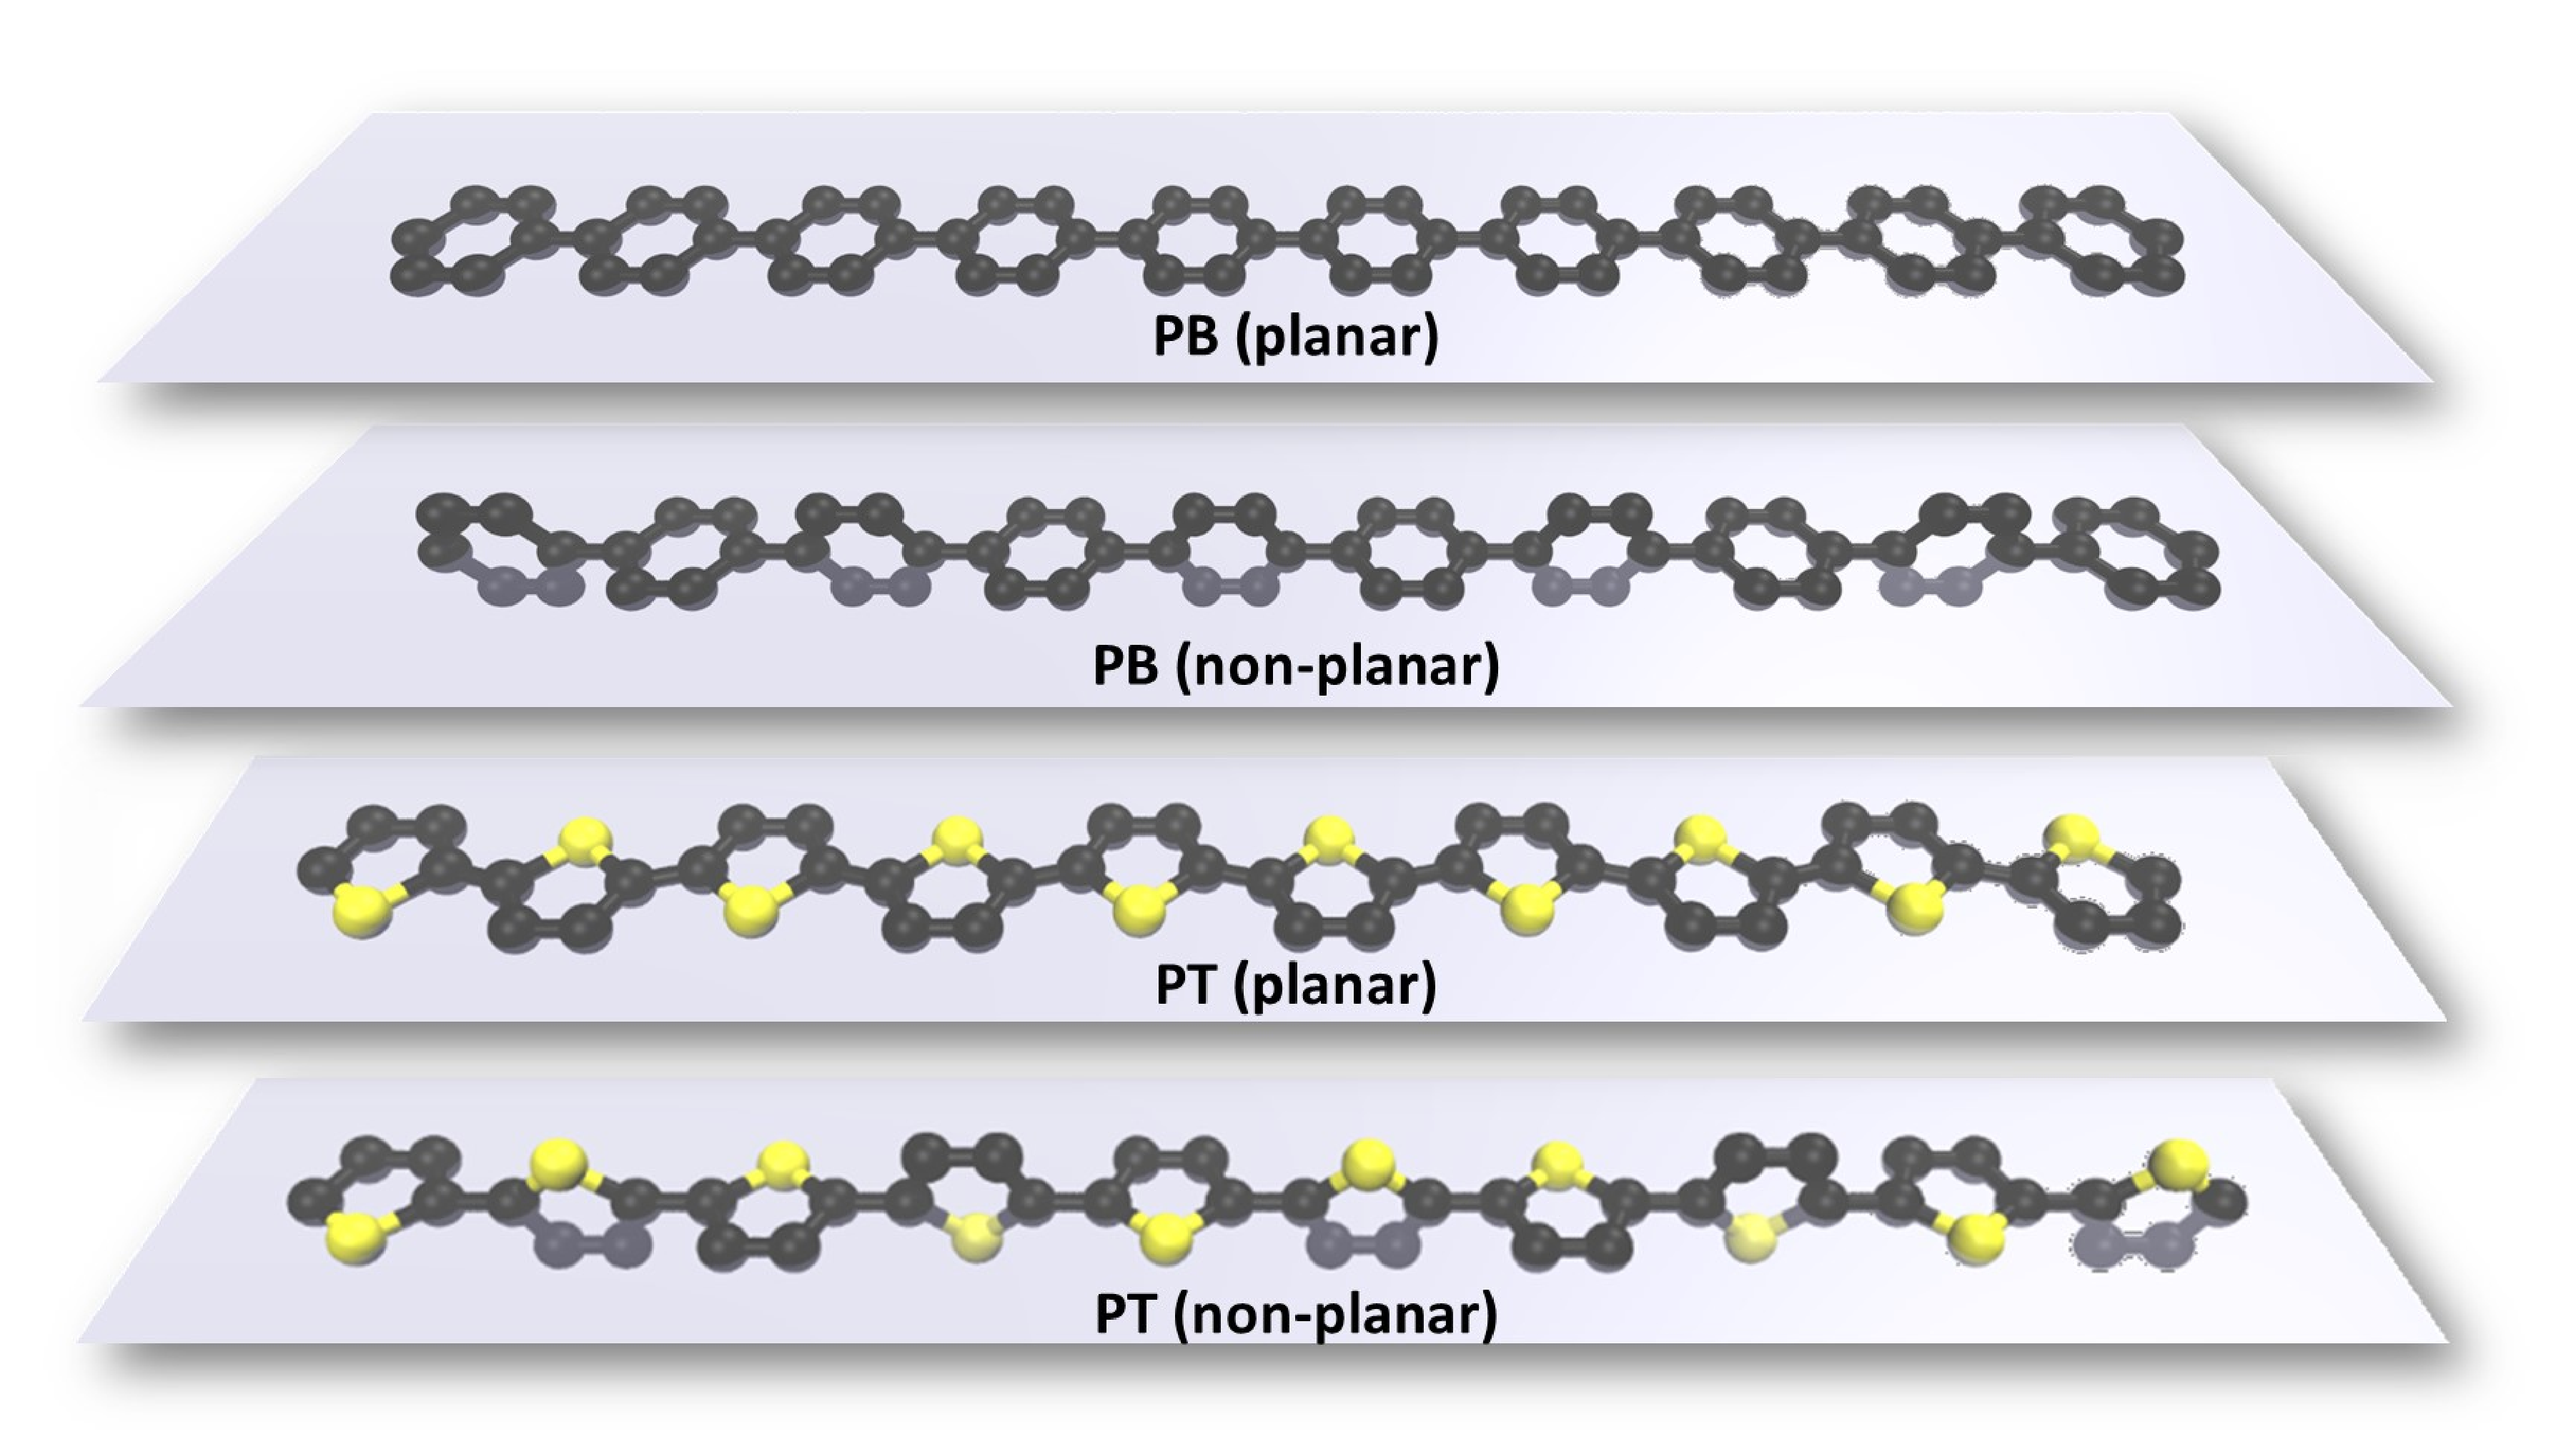
\includegraphics[width=0.744\textwidth]{Chapter-3/Figures/PB_PT_structure.eps}
	\caption{Representation of planar/non-planar structures of PB and PT with a chain length of 10.} 
	\label{fig:PB_PT_structure} 
\end{figure}  

% TODO: get citations from previous papers

%Explain briefly different methods used for benchmarking the polarizability of polymers.
The values of polarizability are generally dependent on DFT approximation and different model chemistries will give different results. In our previous work, we used PBE0/def2-TZVP to calculate polarizability of polymers, but a benchmarking study is necessary to determine a more rational method towards polarizability calculation. Therefore, in this study, polarizability of the polymers is calculated using six different functionals including BP86, PBE0, TPSSh, M06-2X, B2PLYP, and B3LYP. Each of these functionals was used with two def2 basis sets by the Karlsruhe group \cite{Weigend2005}, def2-SVP and def2-TZVP, which are abbreviated as DZ and TZ respectively. Geometry optimization of oligomers is performed at B3LYP/DZ. All the single point calculations as well as the geometry optimizations were performed with D3 correction \cite{Grimme2010}. All the quantum computations are performed using the ORCA quantum chemistry package \cite{Neese2012}.

%Explain the RI model developed for polymers. Lorentz-Lorentz equation and the machine learning model for packing fraction.
The RI of polymers is calculated based on the Lorentz-Lorenz equation, which includes the calculation of two different properties, polarizability and number density. The former is calculated by the method mentioned above, whereas the latter is calculated based on van der Waals volume and packing fraction. The van der Waals volume of the molecules is calculated using Slonimskii's methods \cite{Slonimskii1970}. However, the critical parameter in number density calculation is the packing fraction of the bulk polymer. The most efficient way of calculating packing fraction is to perform molecular dynamics study, but this approach is computationally expensive, therefore, not a viable option for high-throughput screening studies. In our RI prediction model, we established a machine learning approach using a support vector machine on a training data set compiled from the literature to correlate the polymer structure with their packing fraction. The same method is also used in this work for RI calculation.

%Validating the calculated results using 112 experimental values.
The RI values from different model chemistries is validated by comparing with experimental RI values of 112 polymers. The experimental values of these polymers have been taken from Bicerano, polymerdatabase.com, chemicalbook.com, and scientificpolymer.com \cite{Bicerano2002}. 

%Describe the tools for automating the framework of RI calculation of polymers.
In this work, 112 polymers polarizability values are calculated using 12 different methods. For each polymer, four individual calculations are performed from monomer to tetramer. This leads to a total of 5376 calculations. We performed all these calculations in an automated fashion using \chemhtps. 

%Describe the terminology used for error analysis.
The following abbreviations are used for error analysis terms:
MAPE (mean absolute percentage error),
RMSE (root mean squared deviation),
AE (average error),
MaxE (maximum error),
SPRE (difference of maximum and minimum error),
MAE (mean absolute error),
MARE (mean absolute relative error) and
RMSRE (root mean squared relative error)


\section{Results and Discussion}
\label{sec:results_discussion}

%Polarizability of non-conjugated polymer, polyethylene, comparison of different method for the variation of polarizability with the chain length. Fit to a linear regression model and discuss the trends seen.
In our previous studies, we showed that the polarizability of non-conjugated polymers, calculated at PBE0/TZ level, varies linearly with increasing chain length. Here, we calculate the polarizabilities of polyethylene (PE) using different methods. The plot in fig:\ \ref{fig:PE_per} shows the comparison between different methods. Blue color is for DZ and red for TZ. 

Observations:

i. In all methods, the polarizability values have a linear relationship with the PE oligomer chain length. The initial decrease in the values from monomer to trimer is due to the end effects of the hydrogen.

ii. The polarizability per oligomer of PE converge to a constant value right after trimer. This suggests that for non-conjugated systems, it is sufficient to calculate polarizability until tetramer. 

iii. The calculated polarizability values in the decreasing order of BP86\ $>$ B3LYP\ $>$ TPSSh\ $>$ PBE0\ $>$ M06-2X\ $>$ B2PLYP

It is well known that LGA and GGA functionals significantly overestimate the polarizability values, which is also depicted in these studies. The key to solve the problem of overestimation is to include an exact exchange treatment \cite{Mori-Sanchez2003}. Therefore, the functionals  B3LYP, TPSSh, PBE0 and M06-2X, which include HF treatment predict lower polarizability values. Further, the functionals which include perturbation theory along with HF, \eg\ double hybrid functional B2PLYP, predict much lower polarizability values. 
This benchmarking study will assist in understanding the degree of over-prediction for various lower level methods.

\begin{figure}[htbp] 
	\centering
	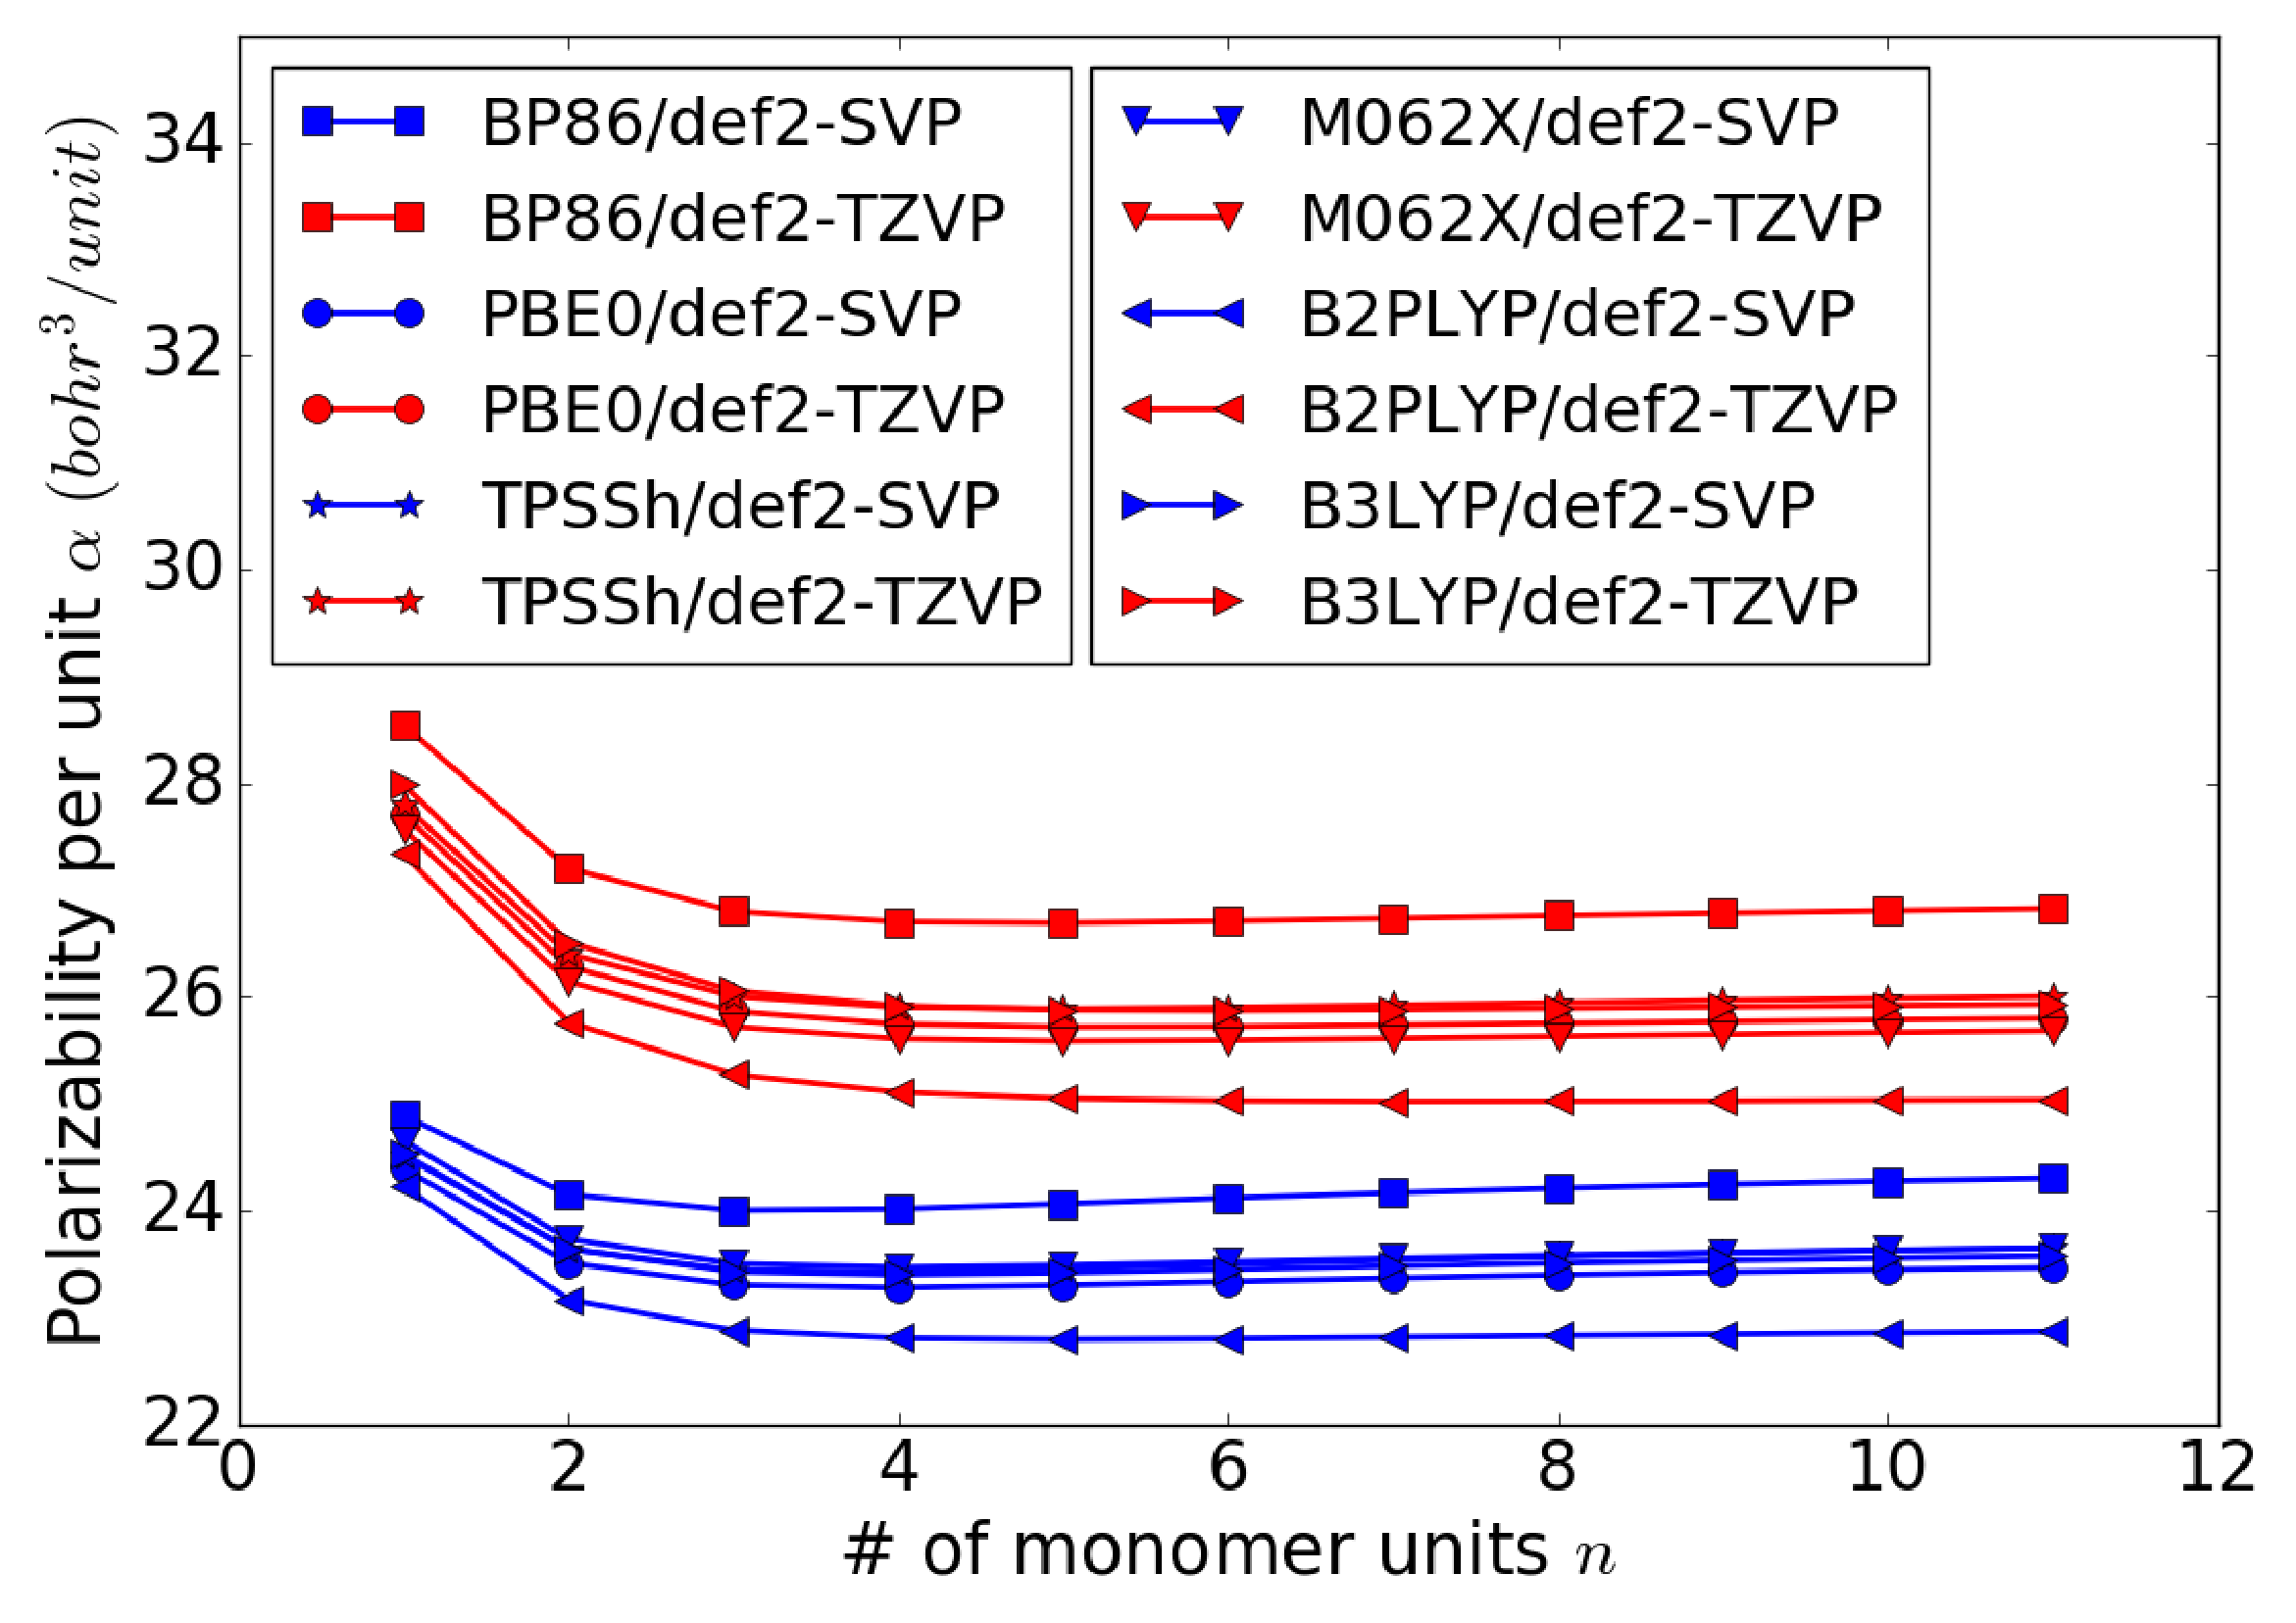
\includegraphics[width=0.744\textwidth]{Chapter-3/Figures/PE_per.eps}
	\caption{Polarizability per oligomer unit of polyethylene with varying chain length calculated from different model chemistries.} 
	\label{fig:PE_per} 
\end{figure}  

%Repeat the above part for conjugated polymer, polyacytylene. 
For conjugated polymers, polyacetylene (PA) is selected as test polymer. Polarizability with increasing chain length is calculated using different functionals and basis set (see fig:\ \ref{fig:PA_per}). The variation of polarizability follows a non-linear behavior with the increasing oligomer length. This is because, as the length is increasing, the conjugation in the molecule also increases leading to increased polarizability. Non-linear correlation can be used to fit the polarizability variation of conjugated polymers. 

\begin{figure}[htbp] 
	\centering
	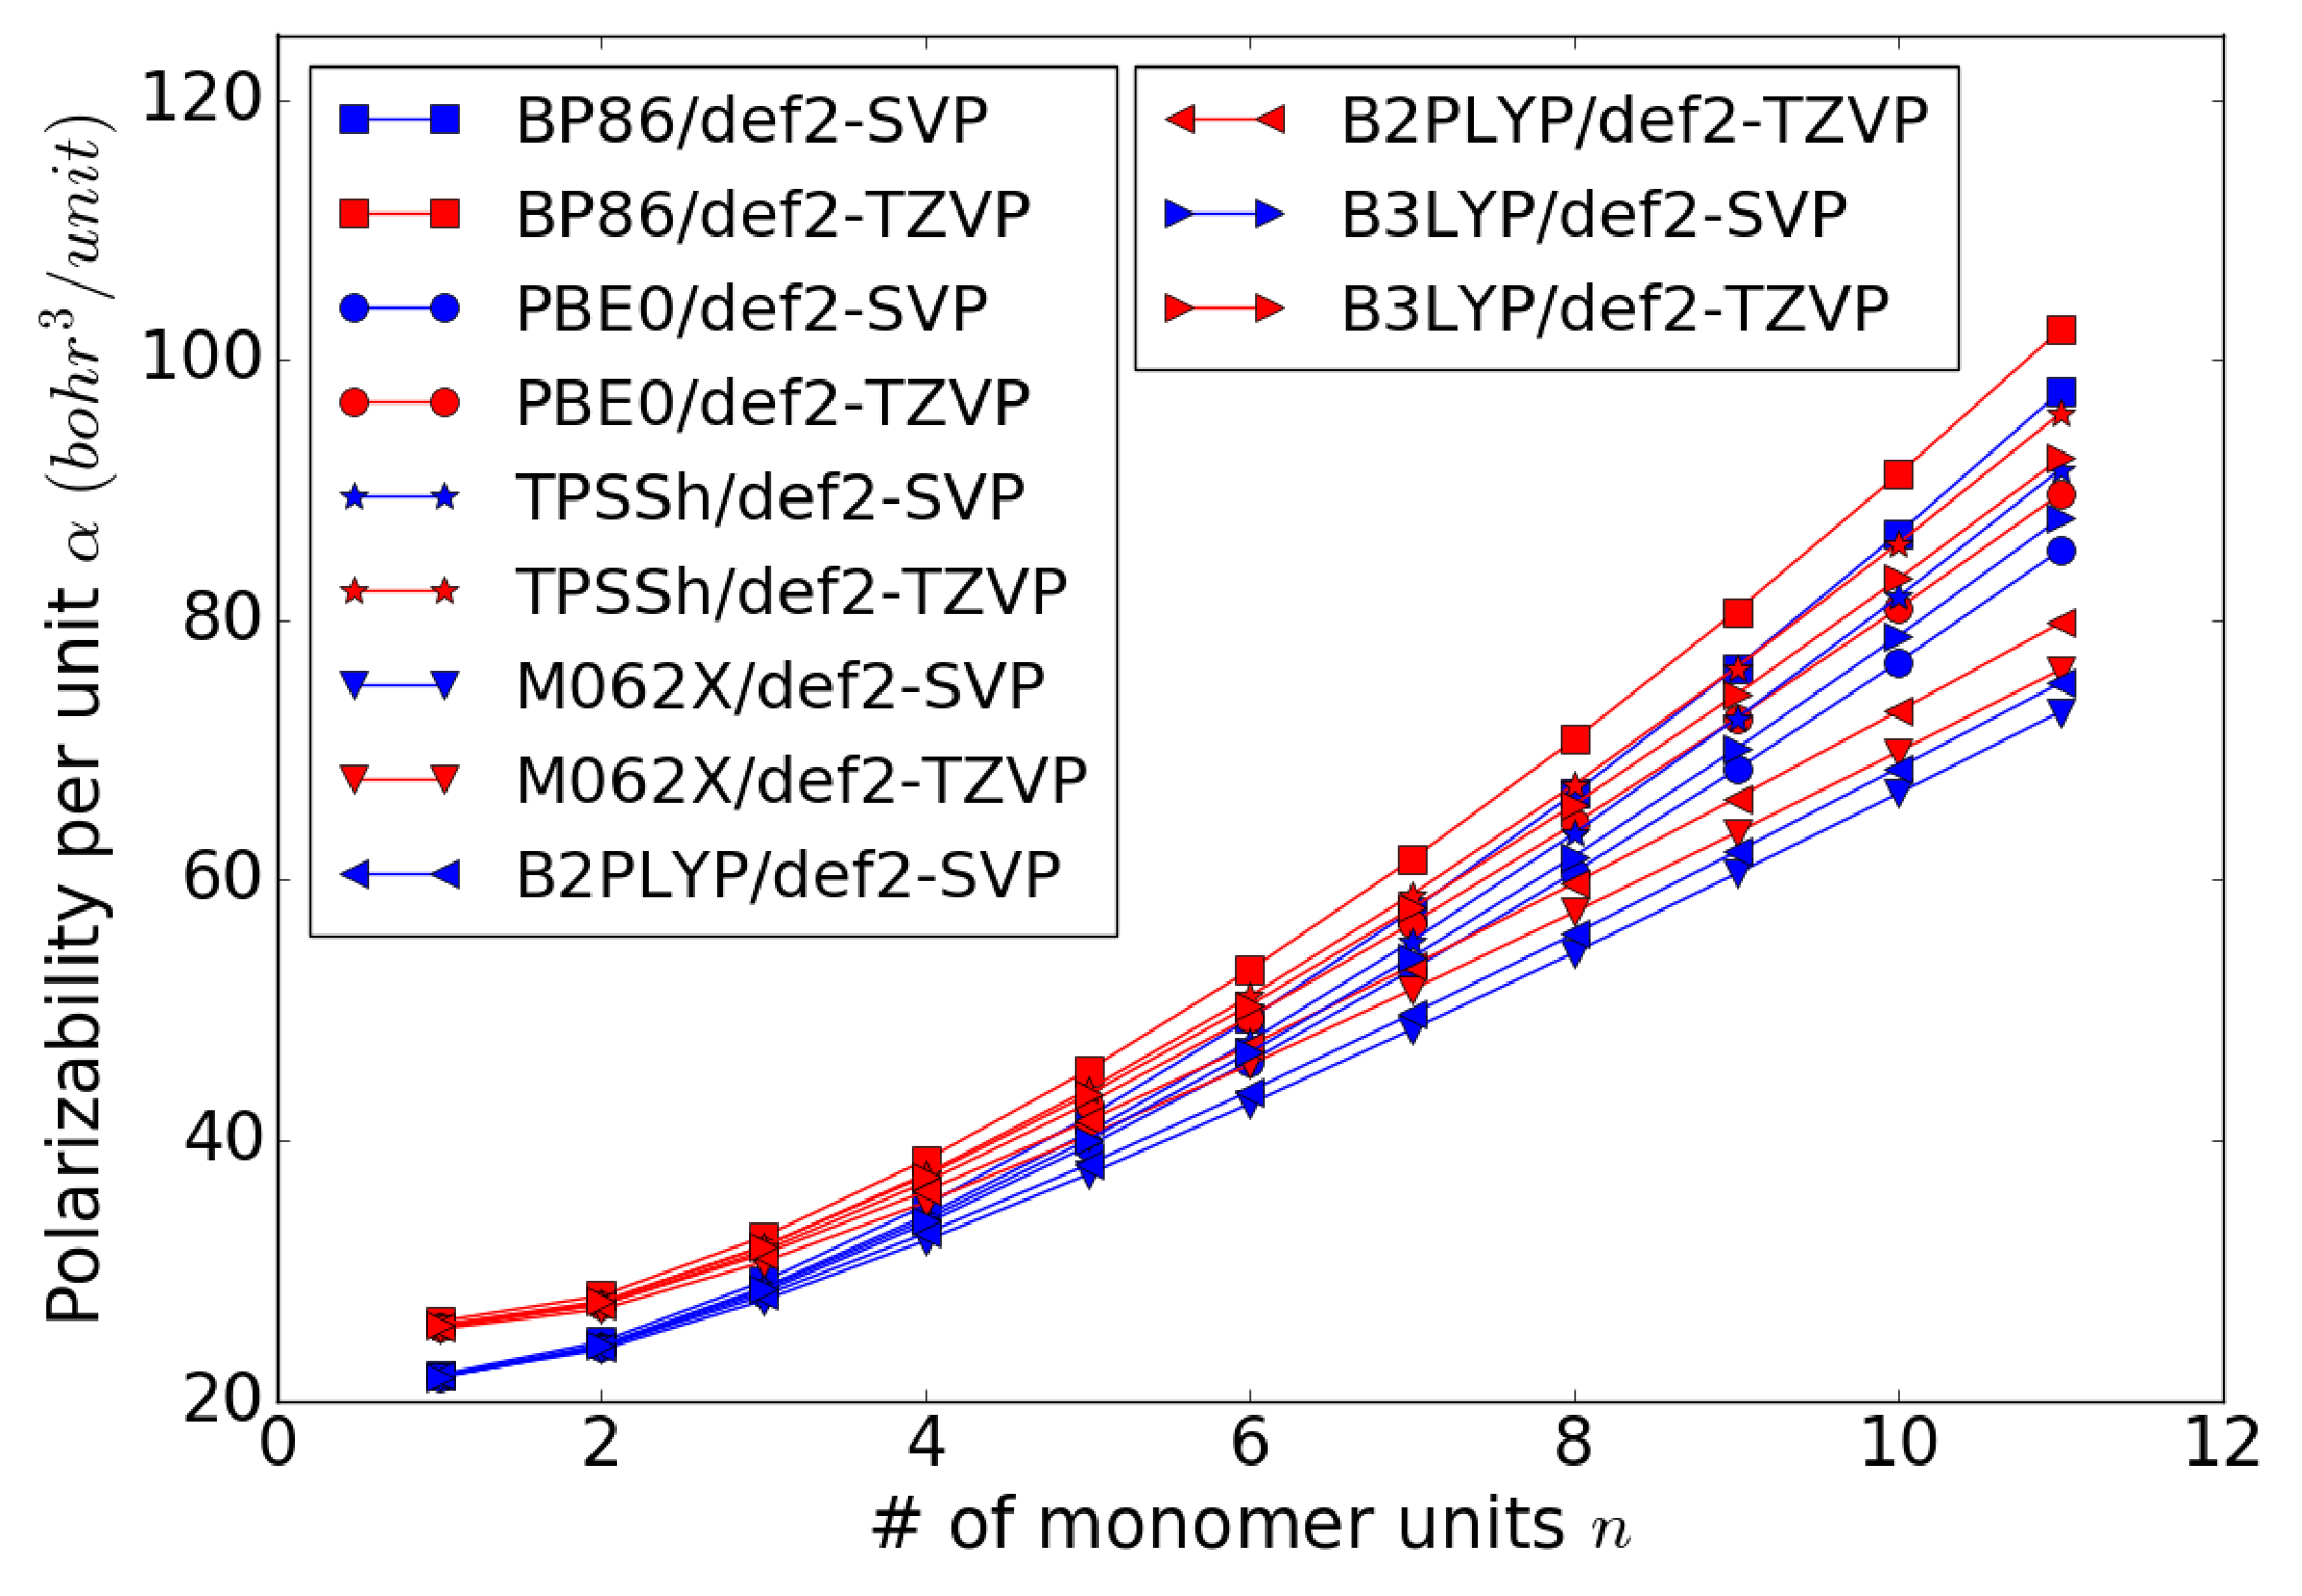
\includegraphics[width=0.744\textwidth]{Chapter-3/Figures/PA_per.eps}
	\caption{Polarizability per oligomer unit of polyacetylene with varying chain length calculated from different model chemistries.} 
	\label{fig:PA_per} 
\end{figure}  

%Comparison of polarizability results when the conjugation is broken by introducing an aliphatic carbon in between. Can also break the conjugation by making non planar molecules.

A better way to compare conjugated and non-conjugated polymers is to break the conjugation by introducing an aliphatic carbon between aromatic rings. For this, two conjugated polymers, PT and PB, are selected and conjugation is broken by introducing non-planarity in the molecule as shown in fig:\ \ref{fig:PB_PT_structure}. The polarizability per oligomer unit increases with chain length for planar PB and PT polymers (see fig:\ fig:\ \ref{fig:C_NC_PB} and fig:\ \ref{fig:C_NC_PT}). For the non-planar PT and PB, the increase in polarizability per oligomer is significantly less. This suggests that the conjugation plays an important role in the polarizability of the polymers. The slight increase of polarizability in non-planar PT and PB shows that there exists a weak conjugation between the aromatic rings. This observation can be better understood by looking at the HOMO and LUMO of PT and PB with a chain length of 5 (see fig:\ \ref{fig:PB_PT_HOMO_LUMO}). The HOMO for planar PB and PT is alternating, suggesting a strong conjugation in the molecule, whereas for non-planar PB and PT, the HOMO is slightly alternating which shows evidence of a weak conjugation. The LUMO distribution of planar PB and PT extends along the full length of molecule, suggesting that the excited electrons would have a clear path to flow. 

\begin{figure}[htbp] 
	\centering
	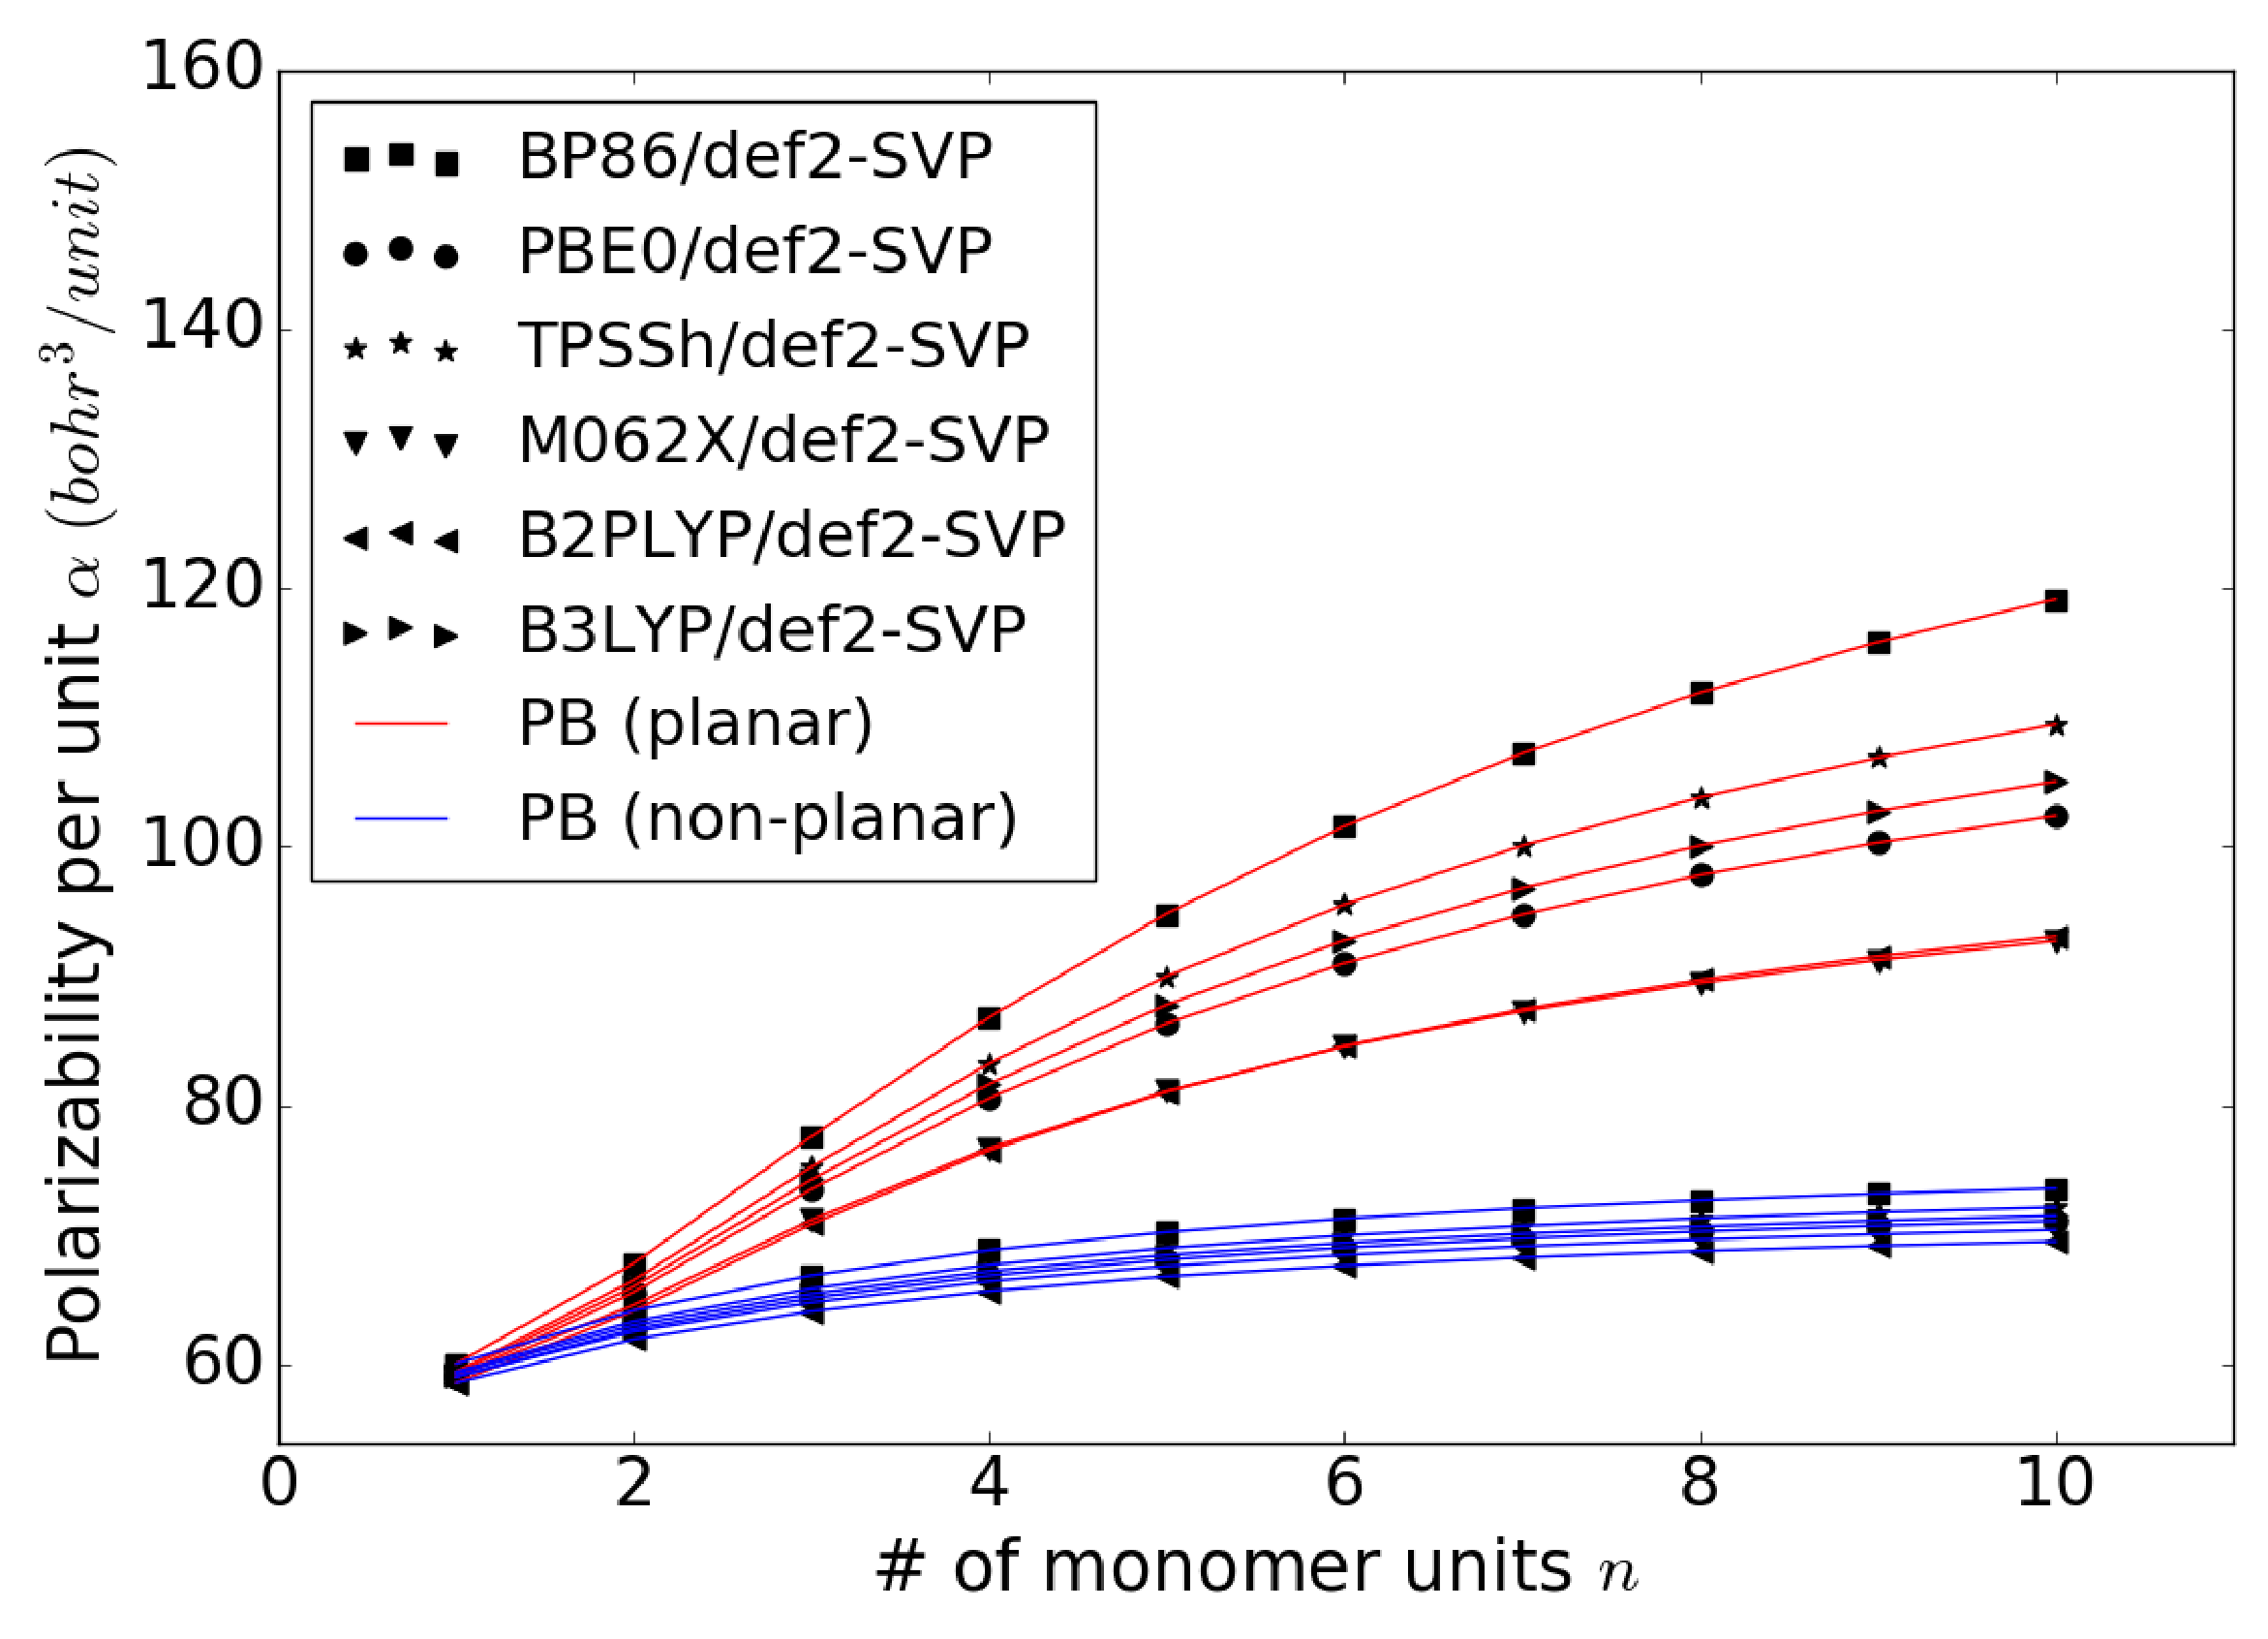
\includegraphics[width=0.744\textwidth]{Chapter-3/Figures/C_NC_PB.eps}
	\caption{Polarizability per oligomer unit of planar and non-planar poly(1,4-phenylene) (PB) with varying chain length calculated from different model chemistries.} 
	\label{fig:C_NC_PB} 
\end{figure}  

\begin{figure}[htbp] 
	\centering
	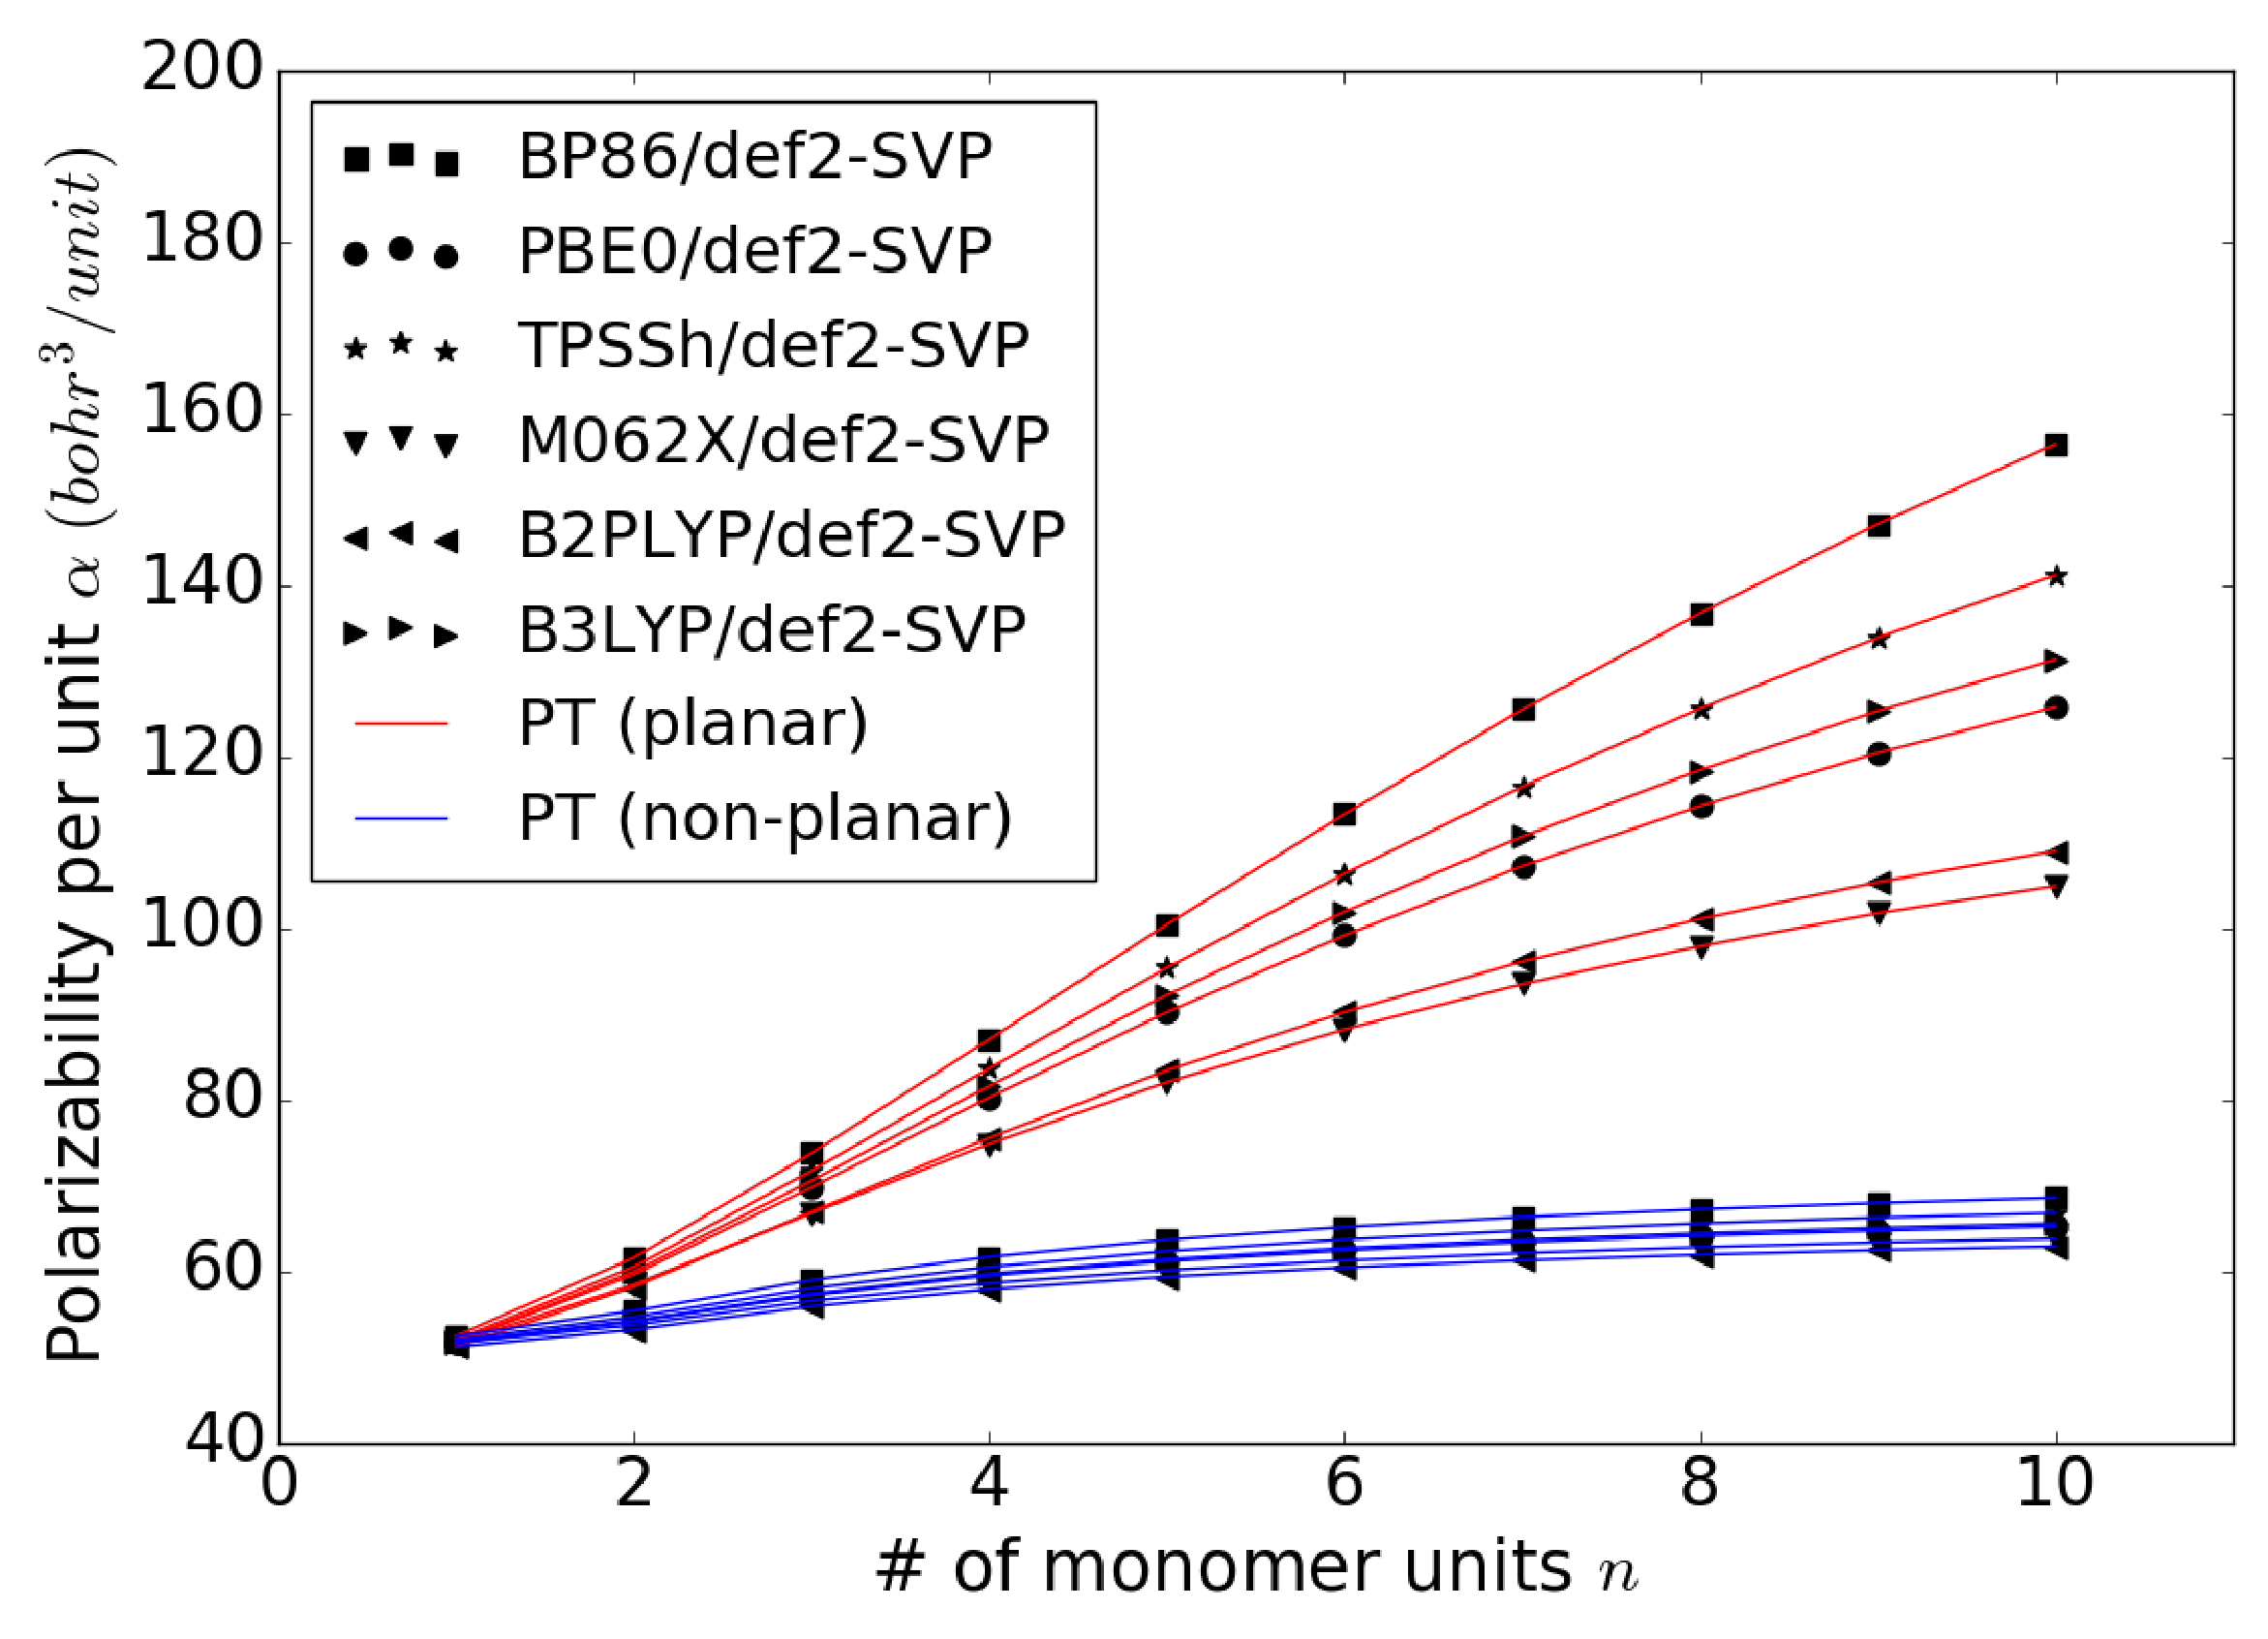
\includegraphics[width=0.744\textwidth]{Chapter-3/Figures/C_NC_PT.eps}
	\caption{Polarizability per oligomer unit of planar and non-planar polythiophene (PT) with varying chain length calculated from different model chemistries.} 
	\label{fig:C_NC_PT} 
\end{figure}  

\begin{figure}[htbp] 
	\centering
	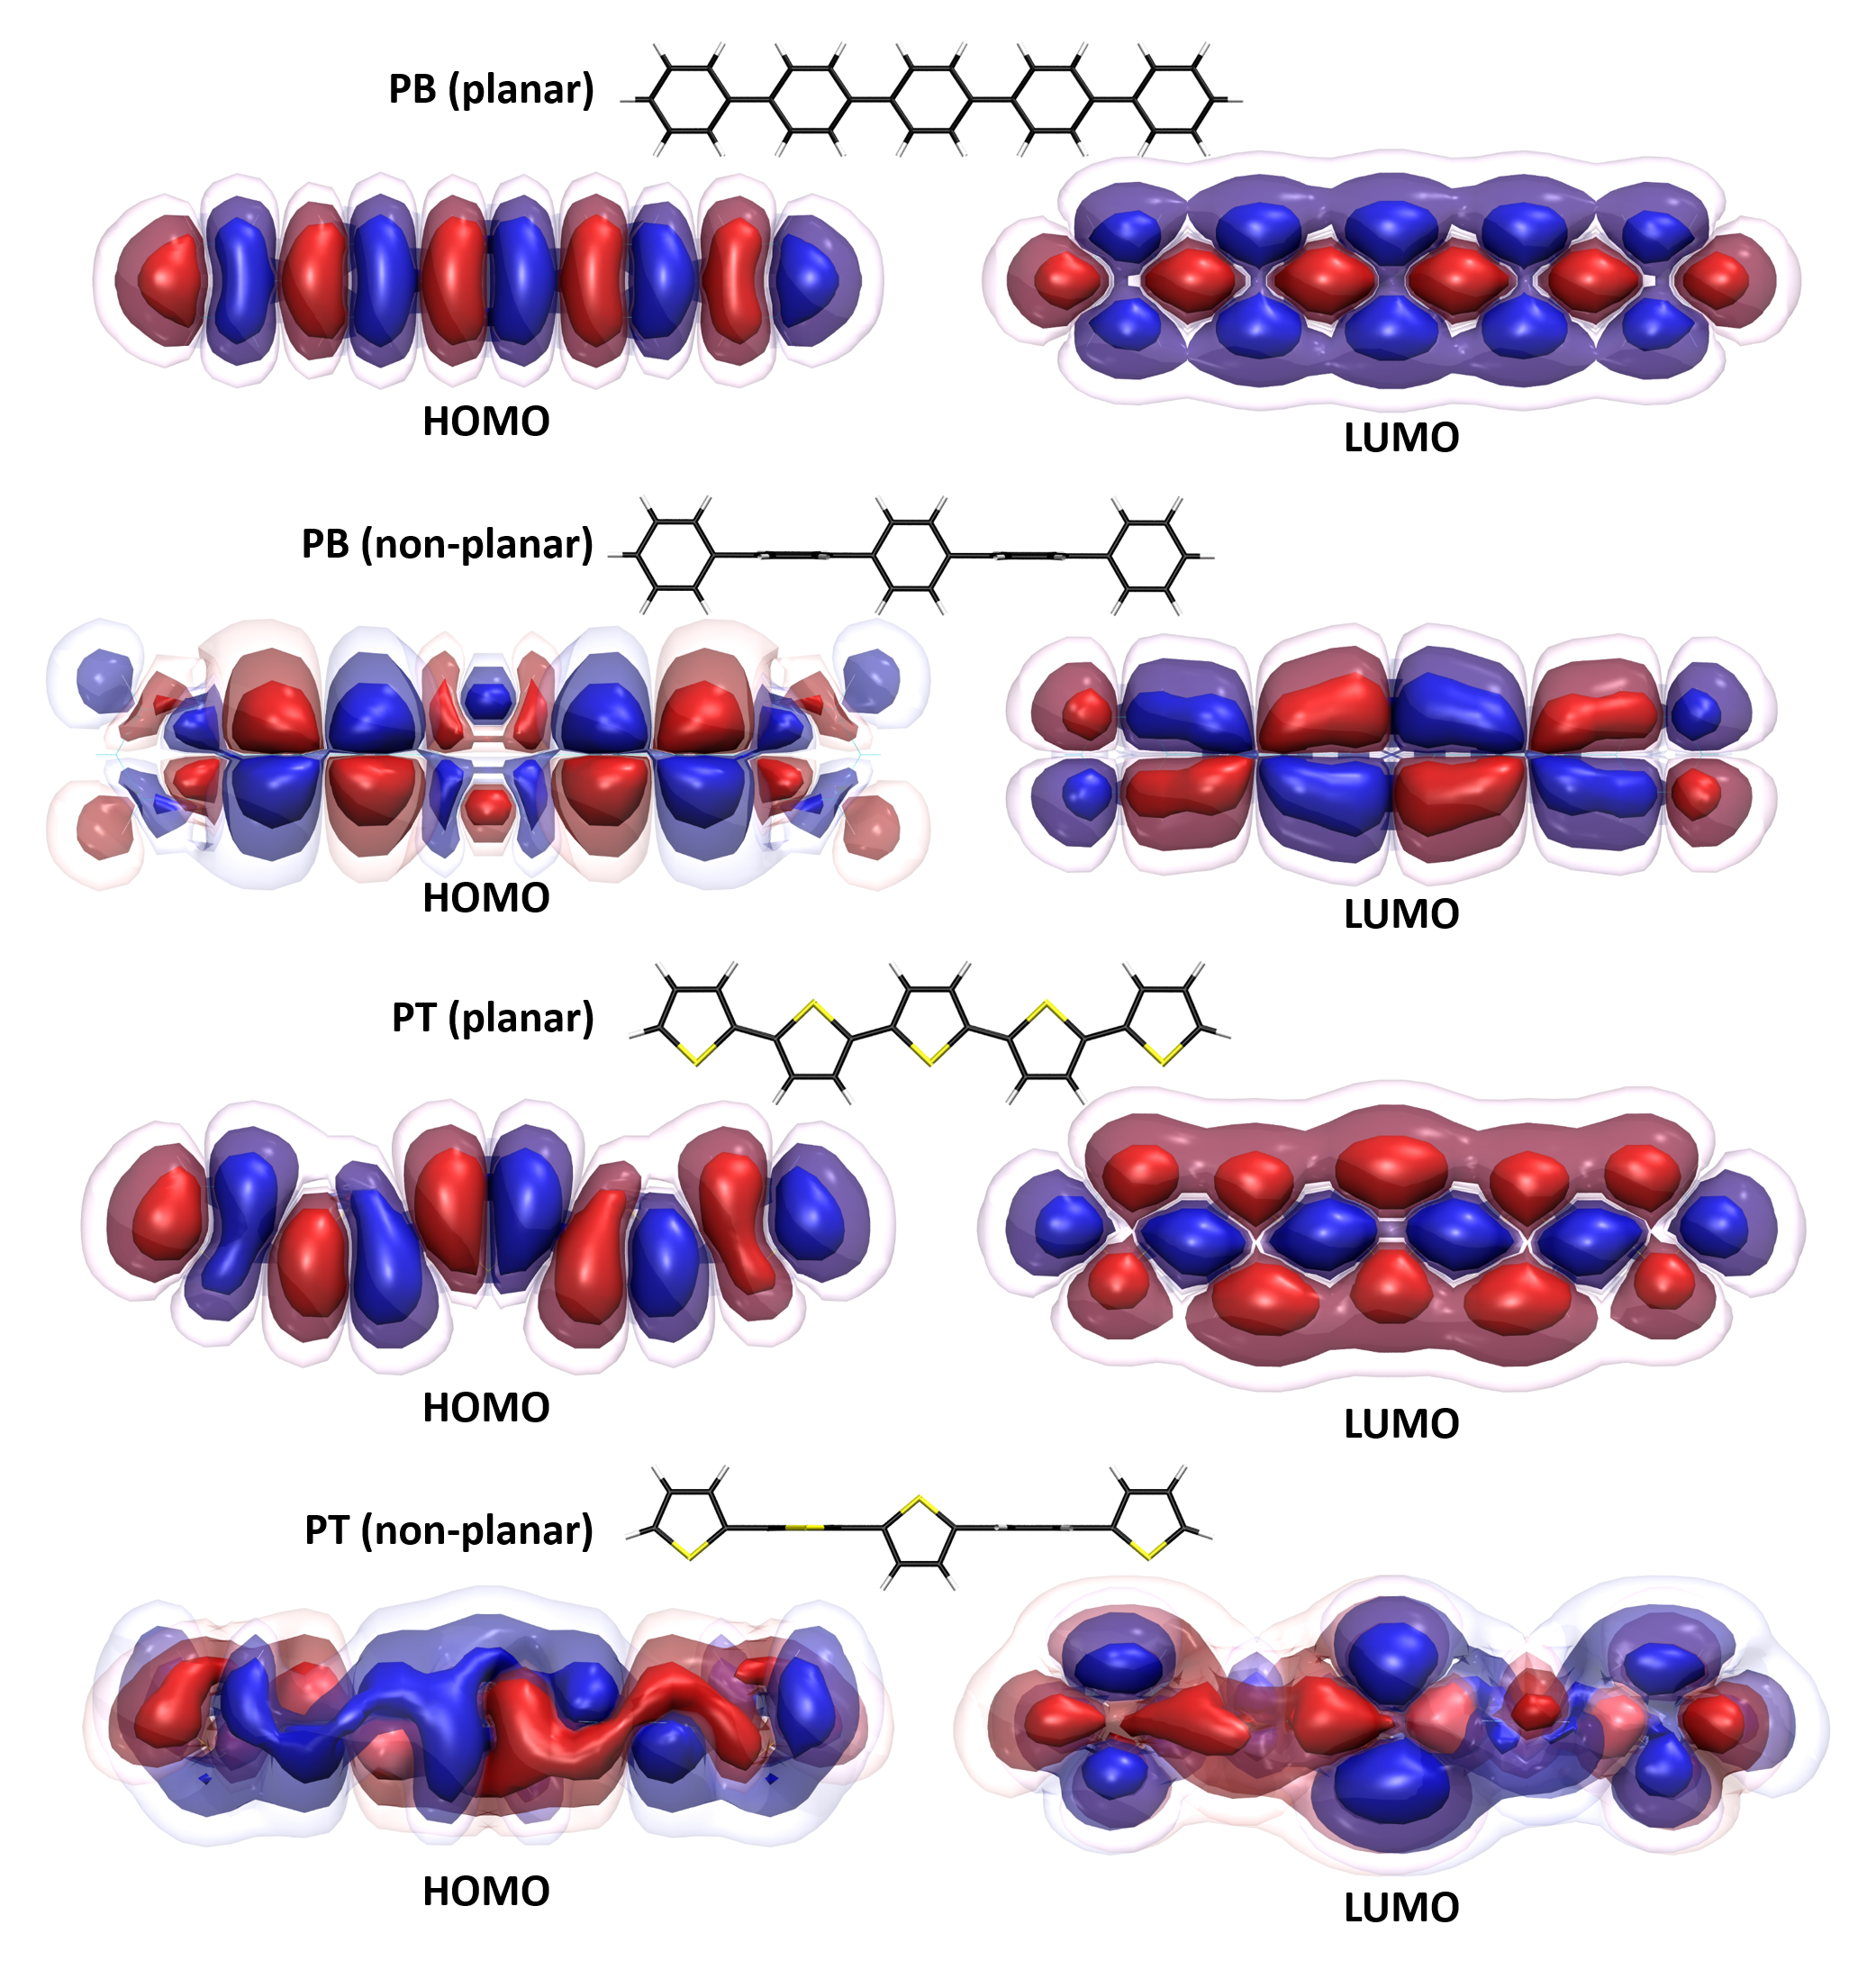
\includegraphics[width=0.744\textwidth]{Chapter-3/Figures/PB_PT_HOMO_LUMO.eps}
	\caption{HOMO (B2PLYP/TZ) and LUMO (B2PLYP/TZ) of planar/non-planar poly(1,4-phenylene) (PB) and polythiophene (PT).} 
	\label{fig:PB_PT_HOMO_LUMO} 
\end{figure}  

%Extrapolation scheme for conjugated polymers. Fit the model to a non-linear equation similar to the equation in Prof. Dupuis paper. Also, find trends.
The variation of polarizability per oligomer unit for conjugated polymers initially increases linearly and then asymptotically converges. A mathematical expression was proposed in literature as shown in the eqn:\ \ref{eqn:1} \cite{Hurst1988}. However, this expression does not fit well for long oligomers (see fig:\ \ref{fig:Pol_fit_all_PBE0_TZ_old}). An extra term is added to the expression as shown in eq:\ \ref{eqn:2}, such that the variation fits well for longer chains (see fig:\ \ref{fig:Pol_fit_all_PBE0_TZ}). This expression is valid for all the three studied conjugated polymers PA, PB and PT. Thus, using this expression, the polarizability of polymer limit can be calculated based on the calculations for small chain oligomers. 

\begin{equation} \label{eqn:1}
\log(\alpha)=a+\frac{b}{N}+\frac{c}{N^2}
\end{equation}


\begin{figure}[htbp] 
	\centering
	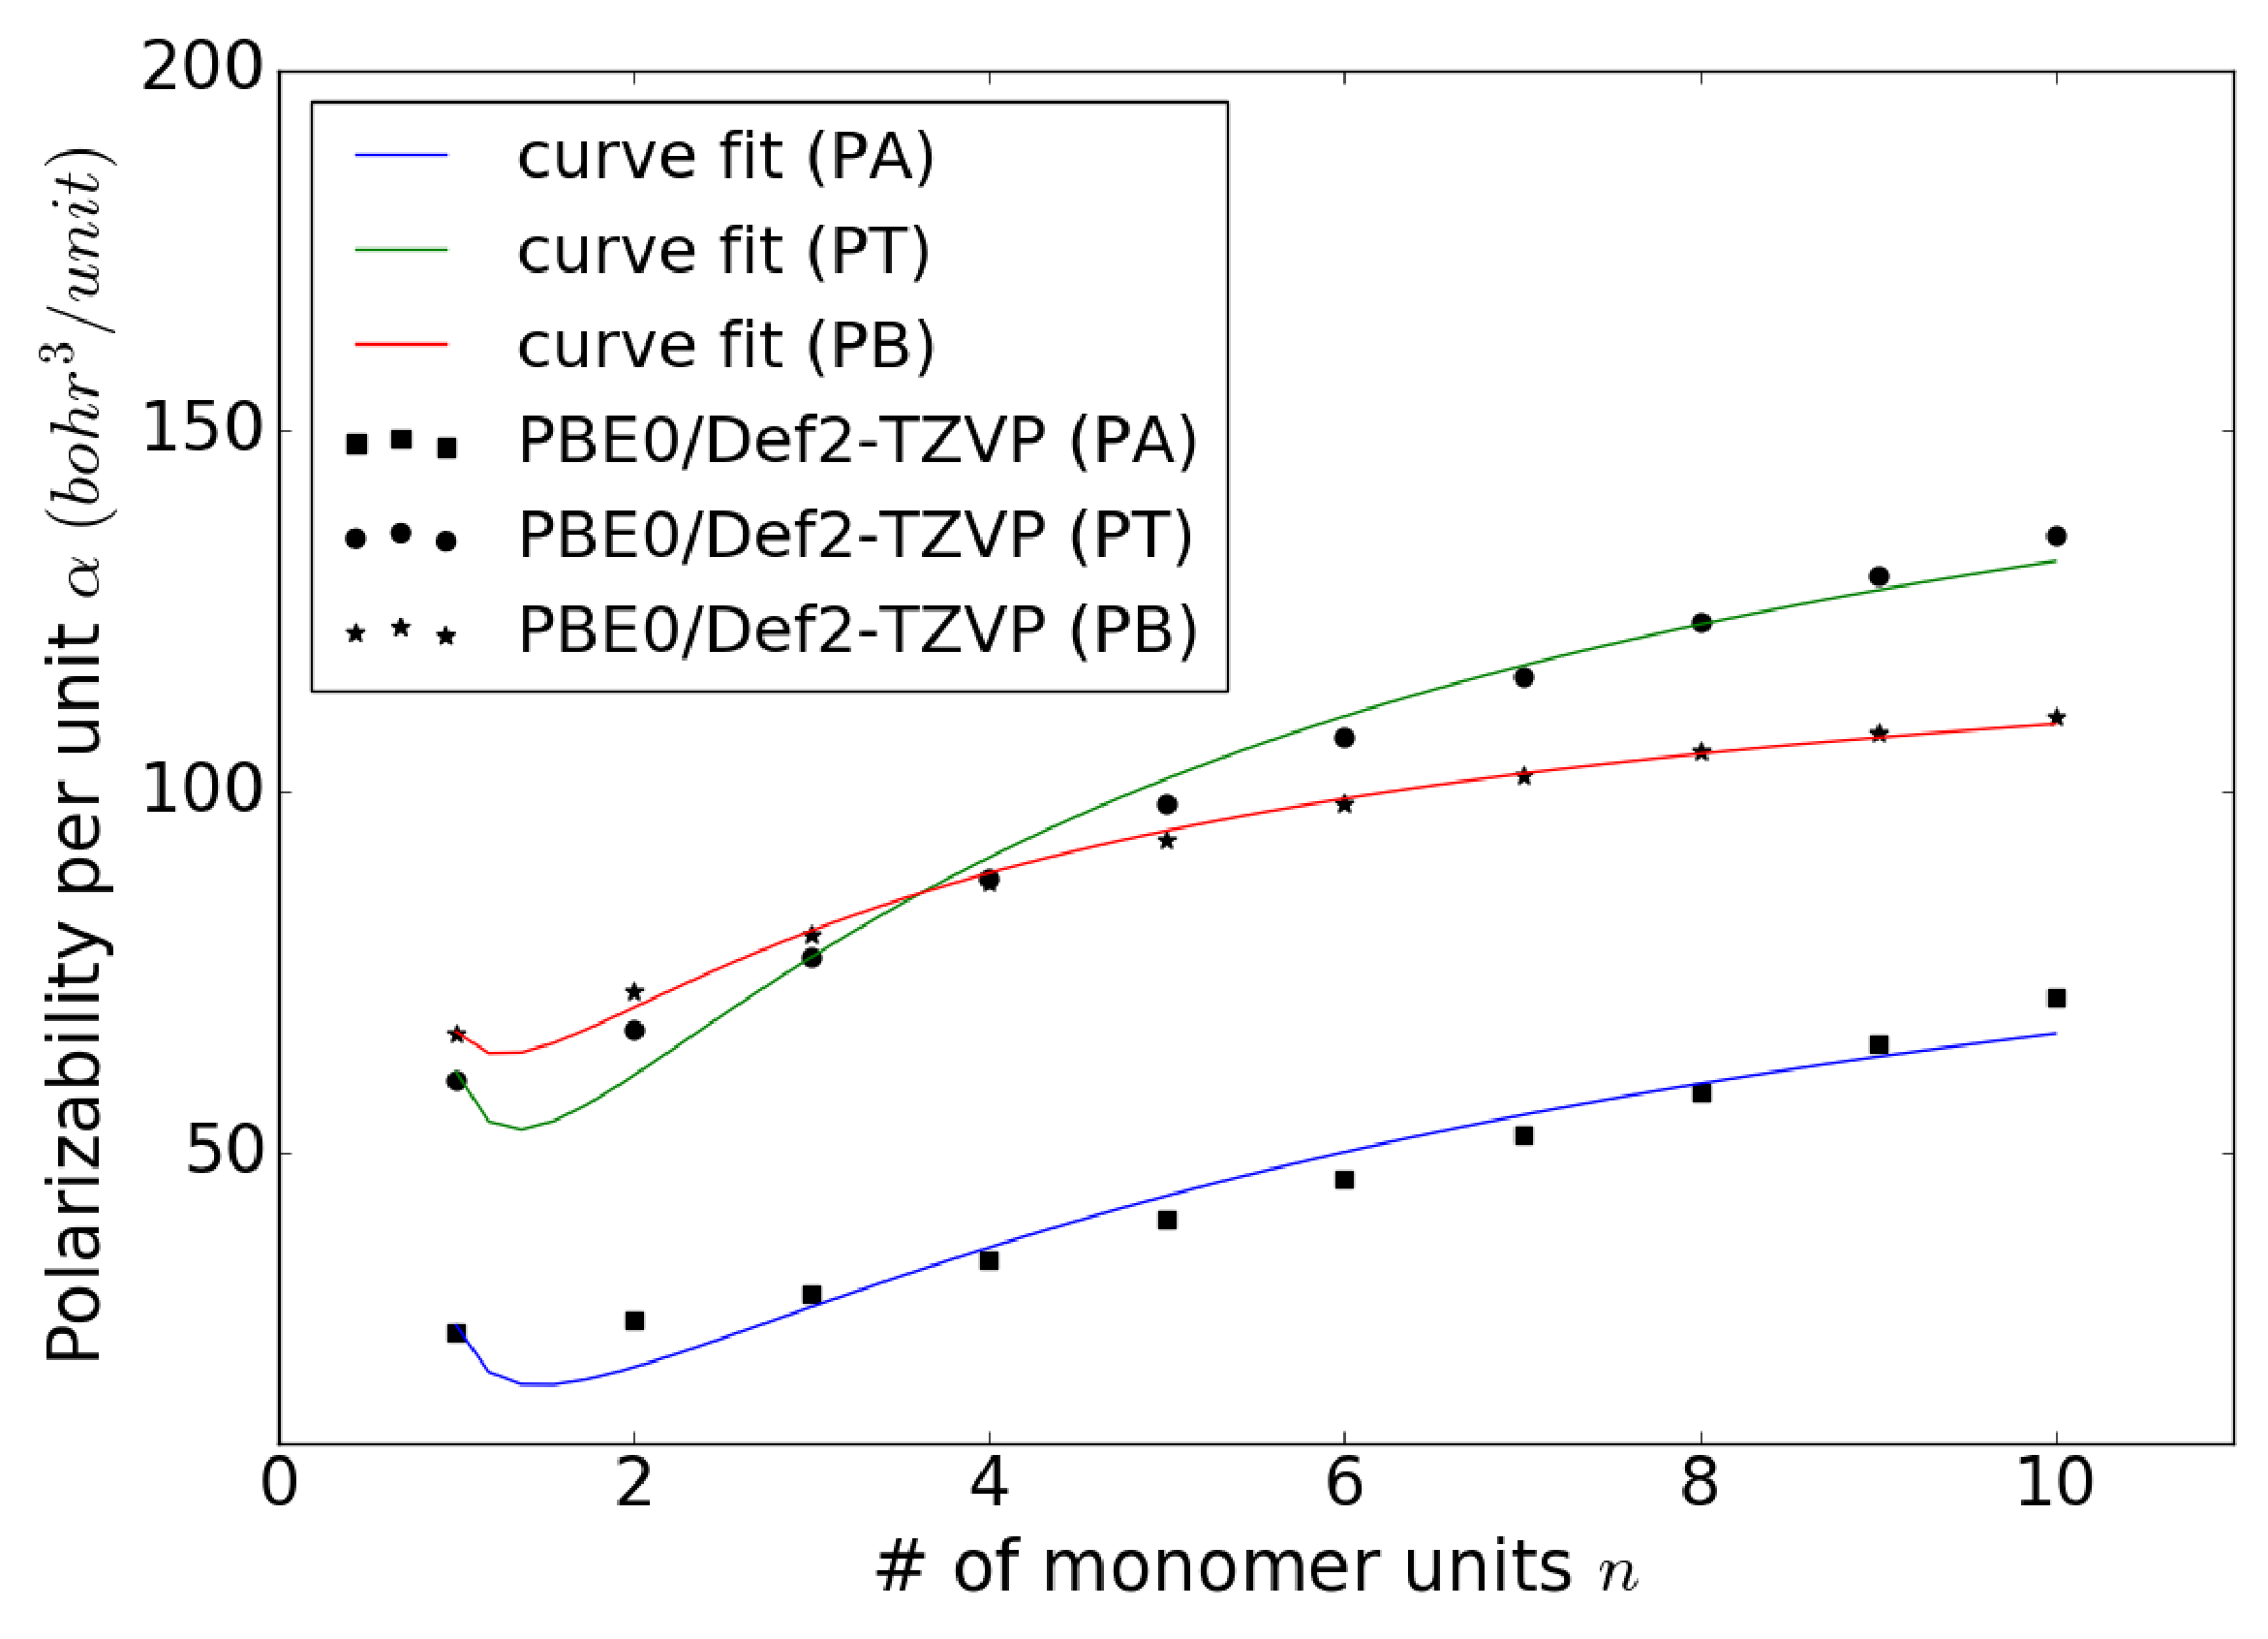
\includegraphics[width=0.744\textwidth]{Chapter-3/Figures/Pol_fit_all_PBE0_TZ_old.eps}
	\caption{Curve fitting using polarizability expression from \cite{Hurst1988} for the conjugated polymers polyacetylene (PA), poly(1,4-phenylene) (PB) and polythiophene (PT). Polarizability is calculated using PBE0/TZ.} 
	\label{fig:Pol_fit_all_PBE0_TZ_old} 
\end{figure}  


\begin{equation} \label{eqn:2}
\log(\alpha)=a+\frac{b}{N}+\frac{c}{N^2}+\frac{d}{N^3}
\end{equation}


\begin{figure}[htbp] 
	\centering
	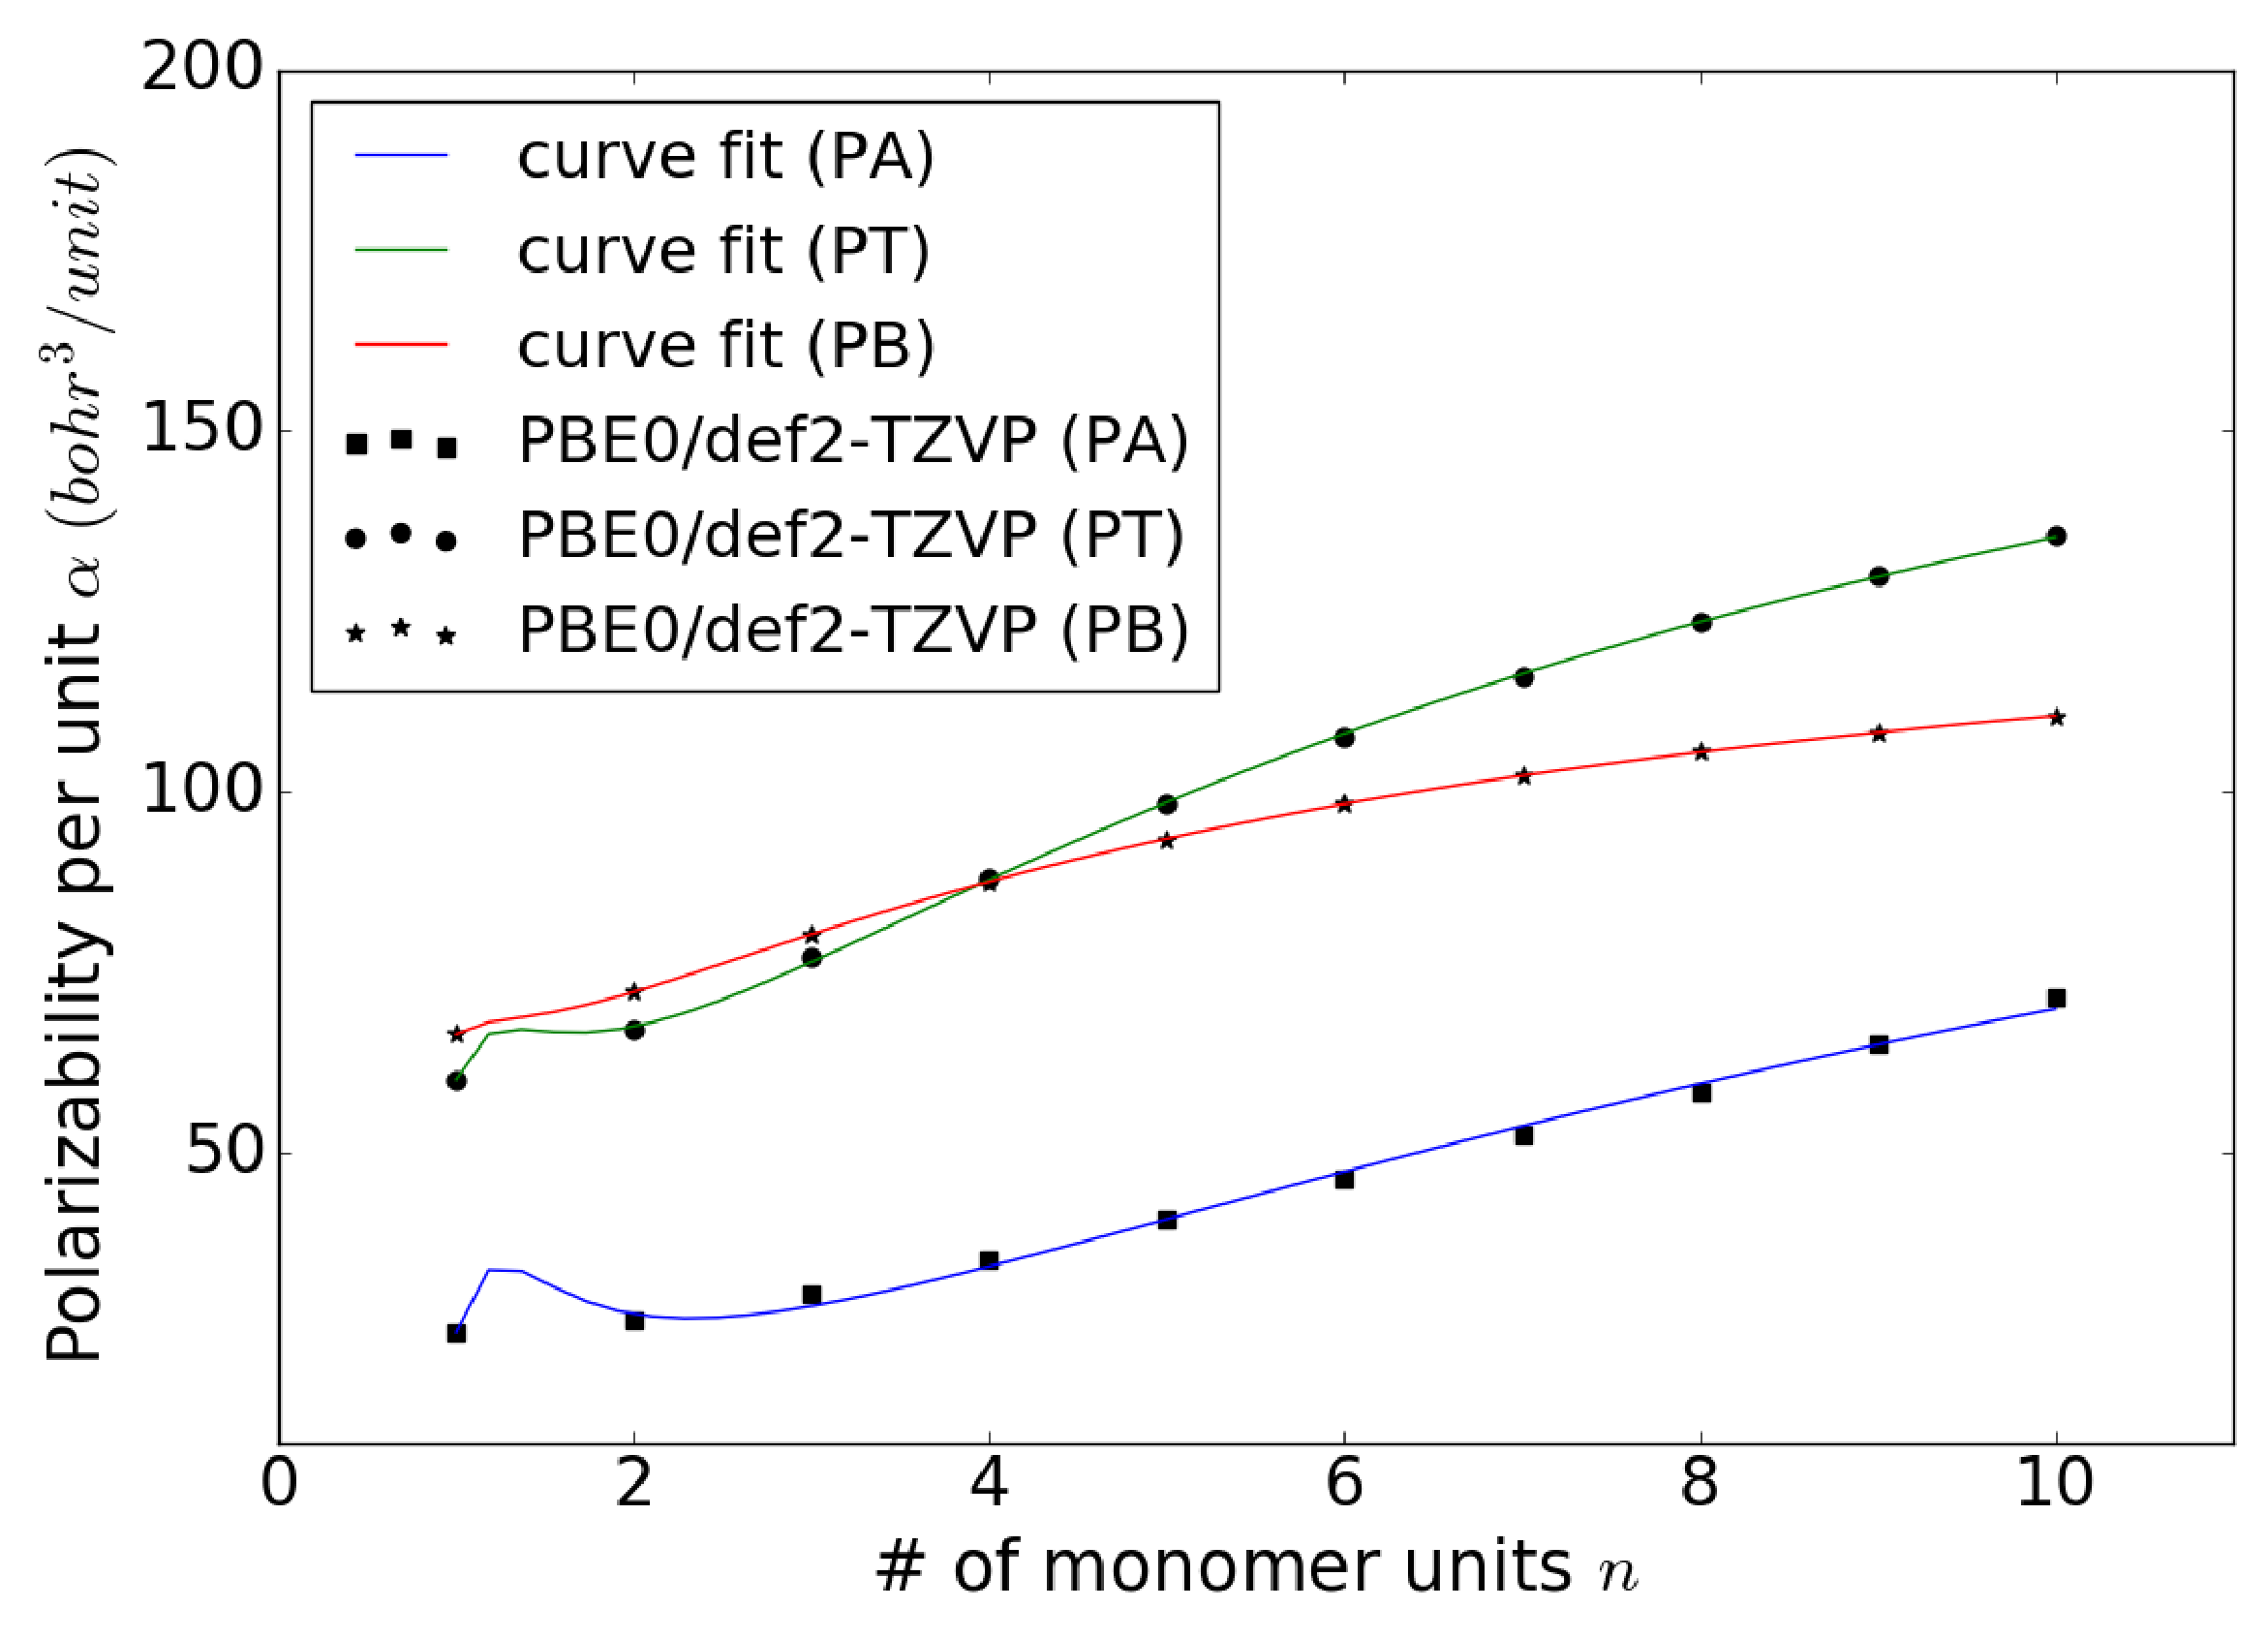
\includegraphics[width=0.744\textwidth]{Chapter-3/Figures/Pol_fit_all_PBE0_TZ.eps}
	\caption{Curve fitting using new polarizability expression for the conjugated polymers polyacetylene (PA), poly(1,4-phenylene) (PB) and polythiophene (PT). Polarizability is calculated using PBE0/TZ.} 
	\label{fig:Pol_fit_all_PBE0_TZ} 
\end{figure}  


%Validation of the extrapolation schemes using longer oligomer chains.
To check the validity of the expression, oligomers up to a chain length of 50 were created. It should be noted that these oligomers were not geometry optimized. The bond lengths and angles were selected based on the optimized geometry of 10 oligomer chain length. We observed that the expression is valid for very long chain lengths (see fig:\ \ref{fig:Pol_fit_all_long_PBE0_DZ}). Using these extrapolation schemes, the polarizability of polymers can be calculated quickly. Further, these schemes are implemented in the high throughput screening framework to accelerate polarizability for large number of polymers. Using the \chemhtps\ framework, the polarizability values of 112 polymers are determined from 12 different methods.

\begin{figure}[htbp] 
	\centering
	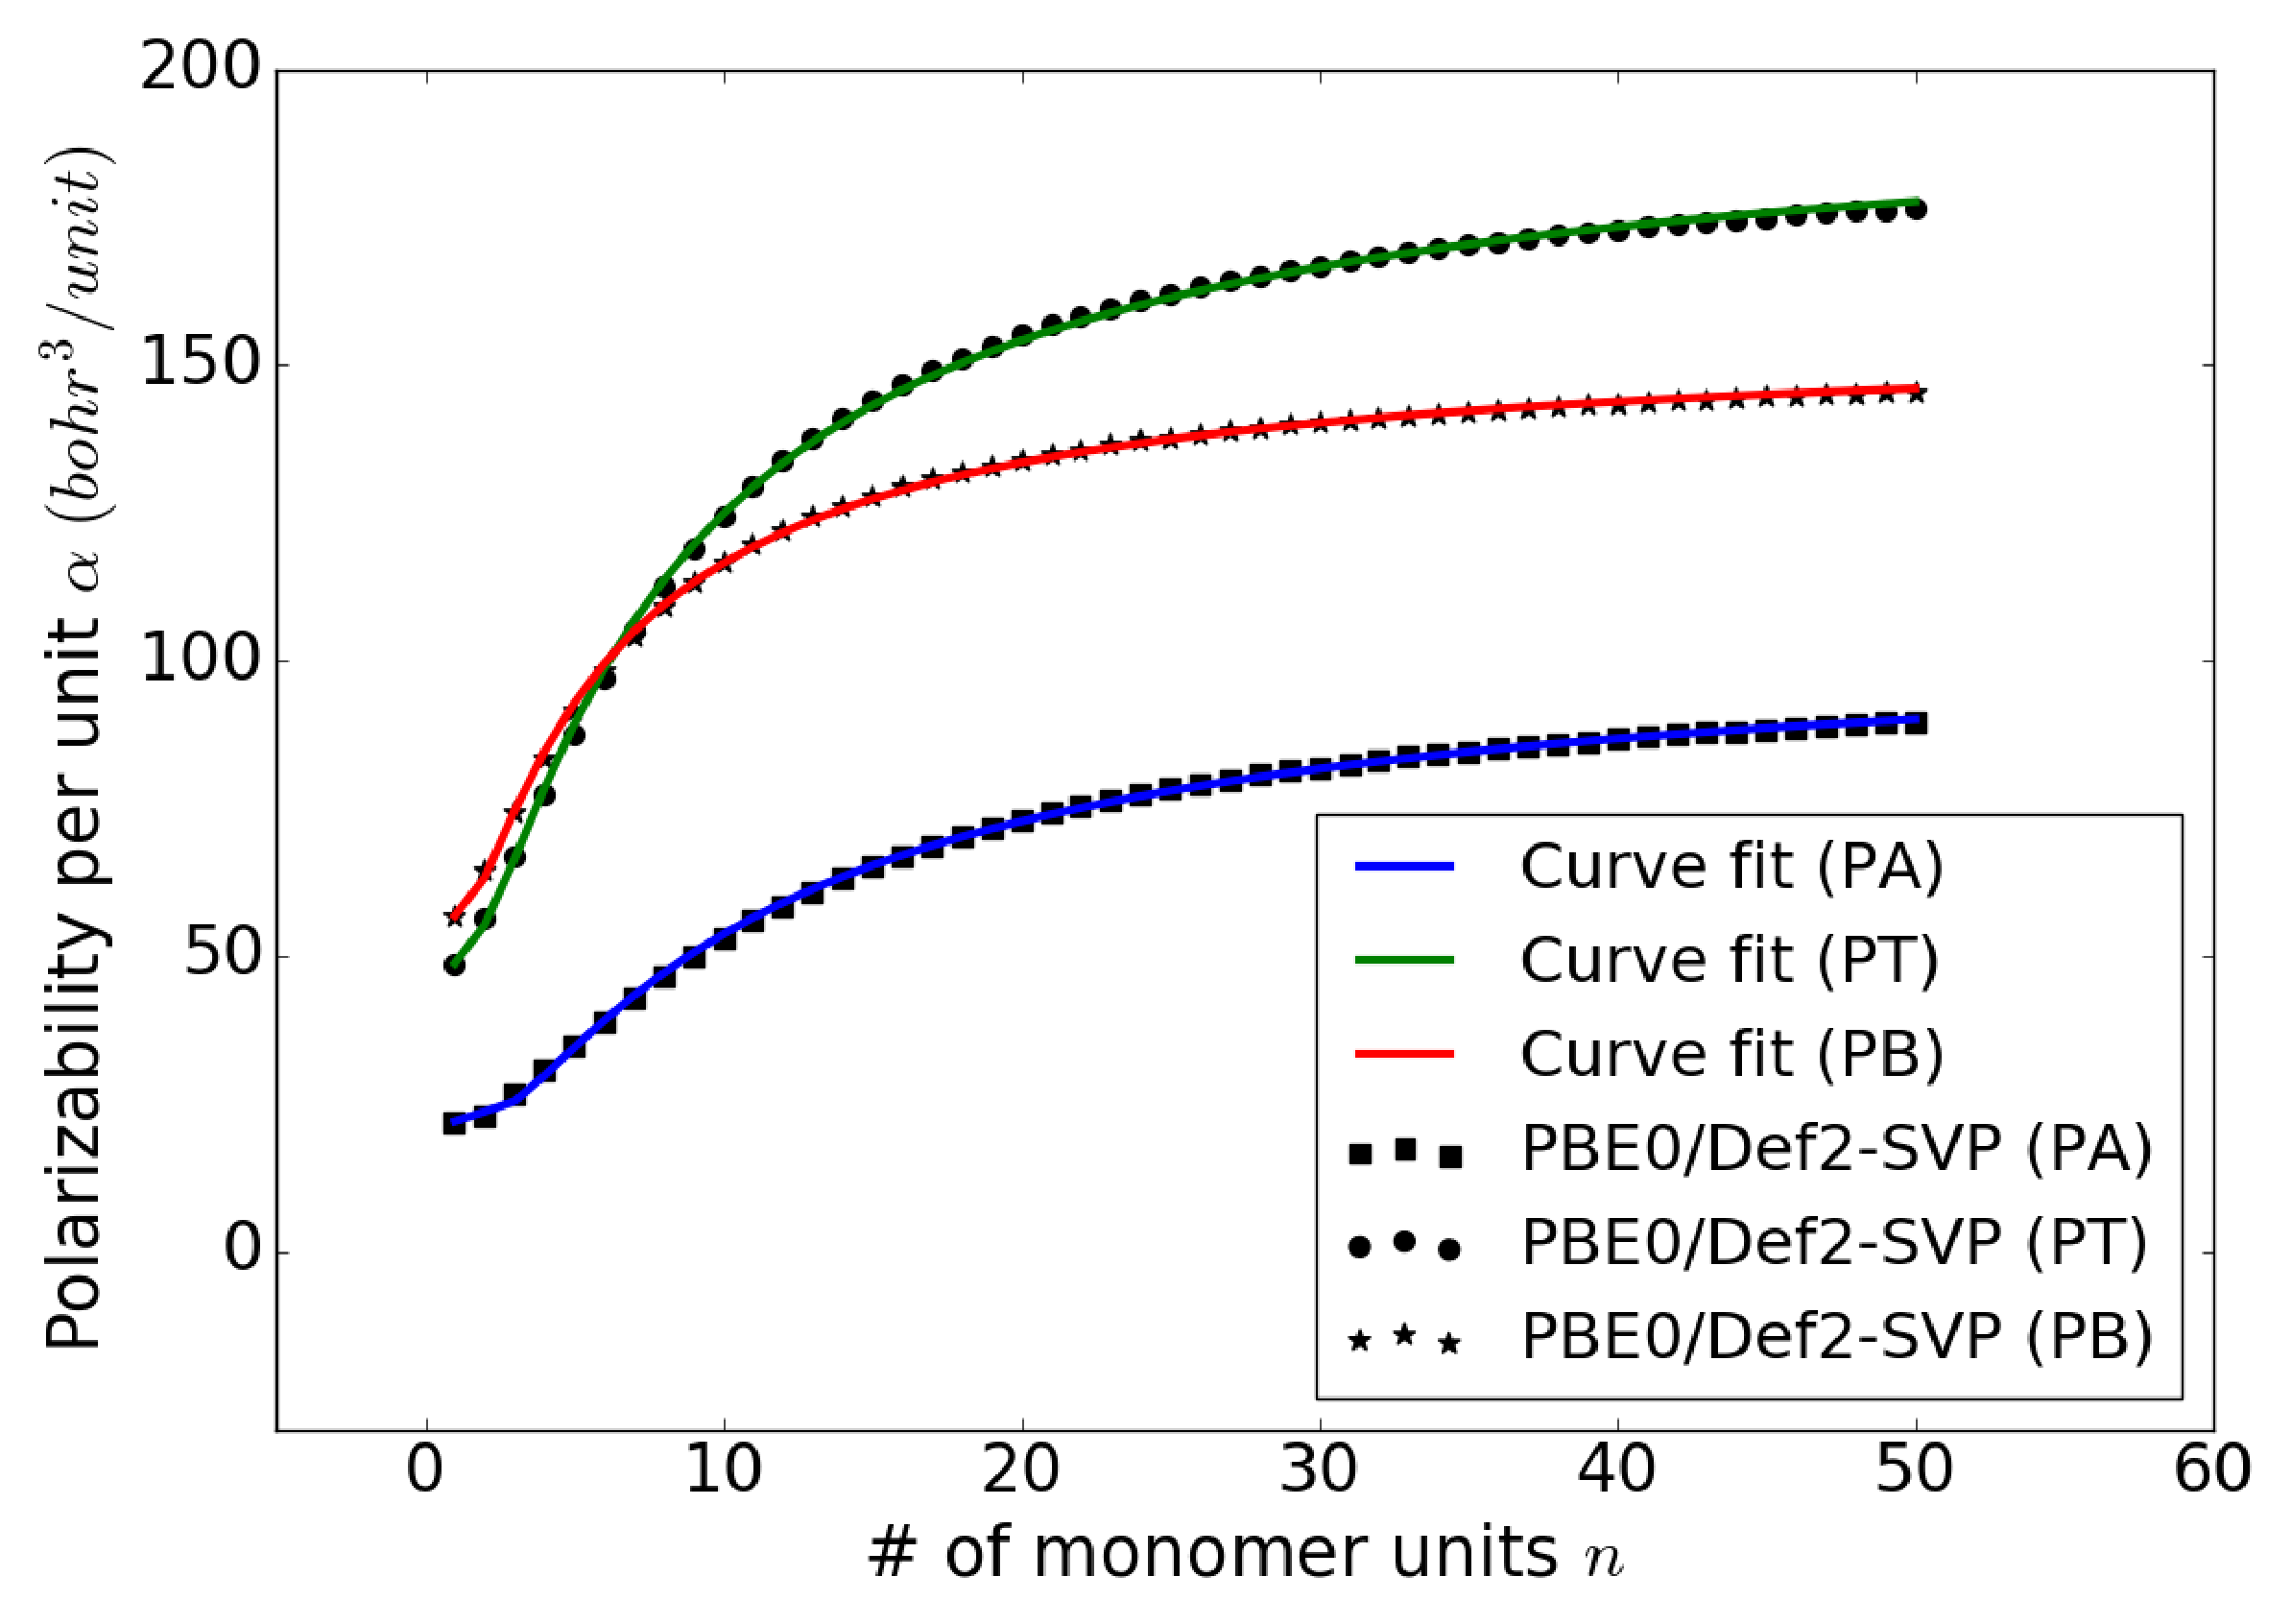
\includegraphics[width=0.744\textwidth]{Chapter-3/Figures/Pol_fit_all_long_PBE0_DZ.eps}
	\caption{Validation of the polarizability expression for long chain lengths of polyacetylene (PA), poly(1,4-phenylene) (PB) and polythiophene (PT). Polarizability calculated using PBE0/DZ} 
	\label{fig:Pol_fit_all_long_PBE0_DZ} 
\end{figure}  

\begin{figure}[htbp] 
	\centering
	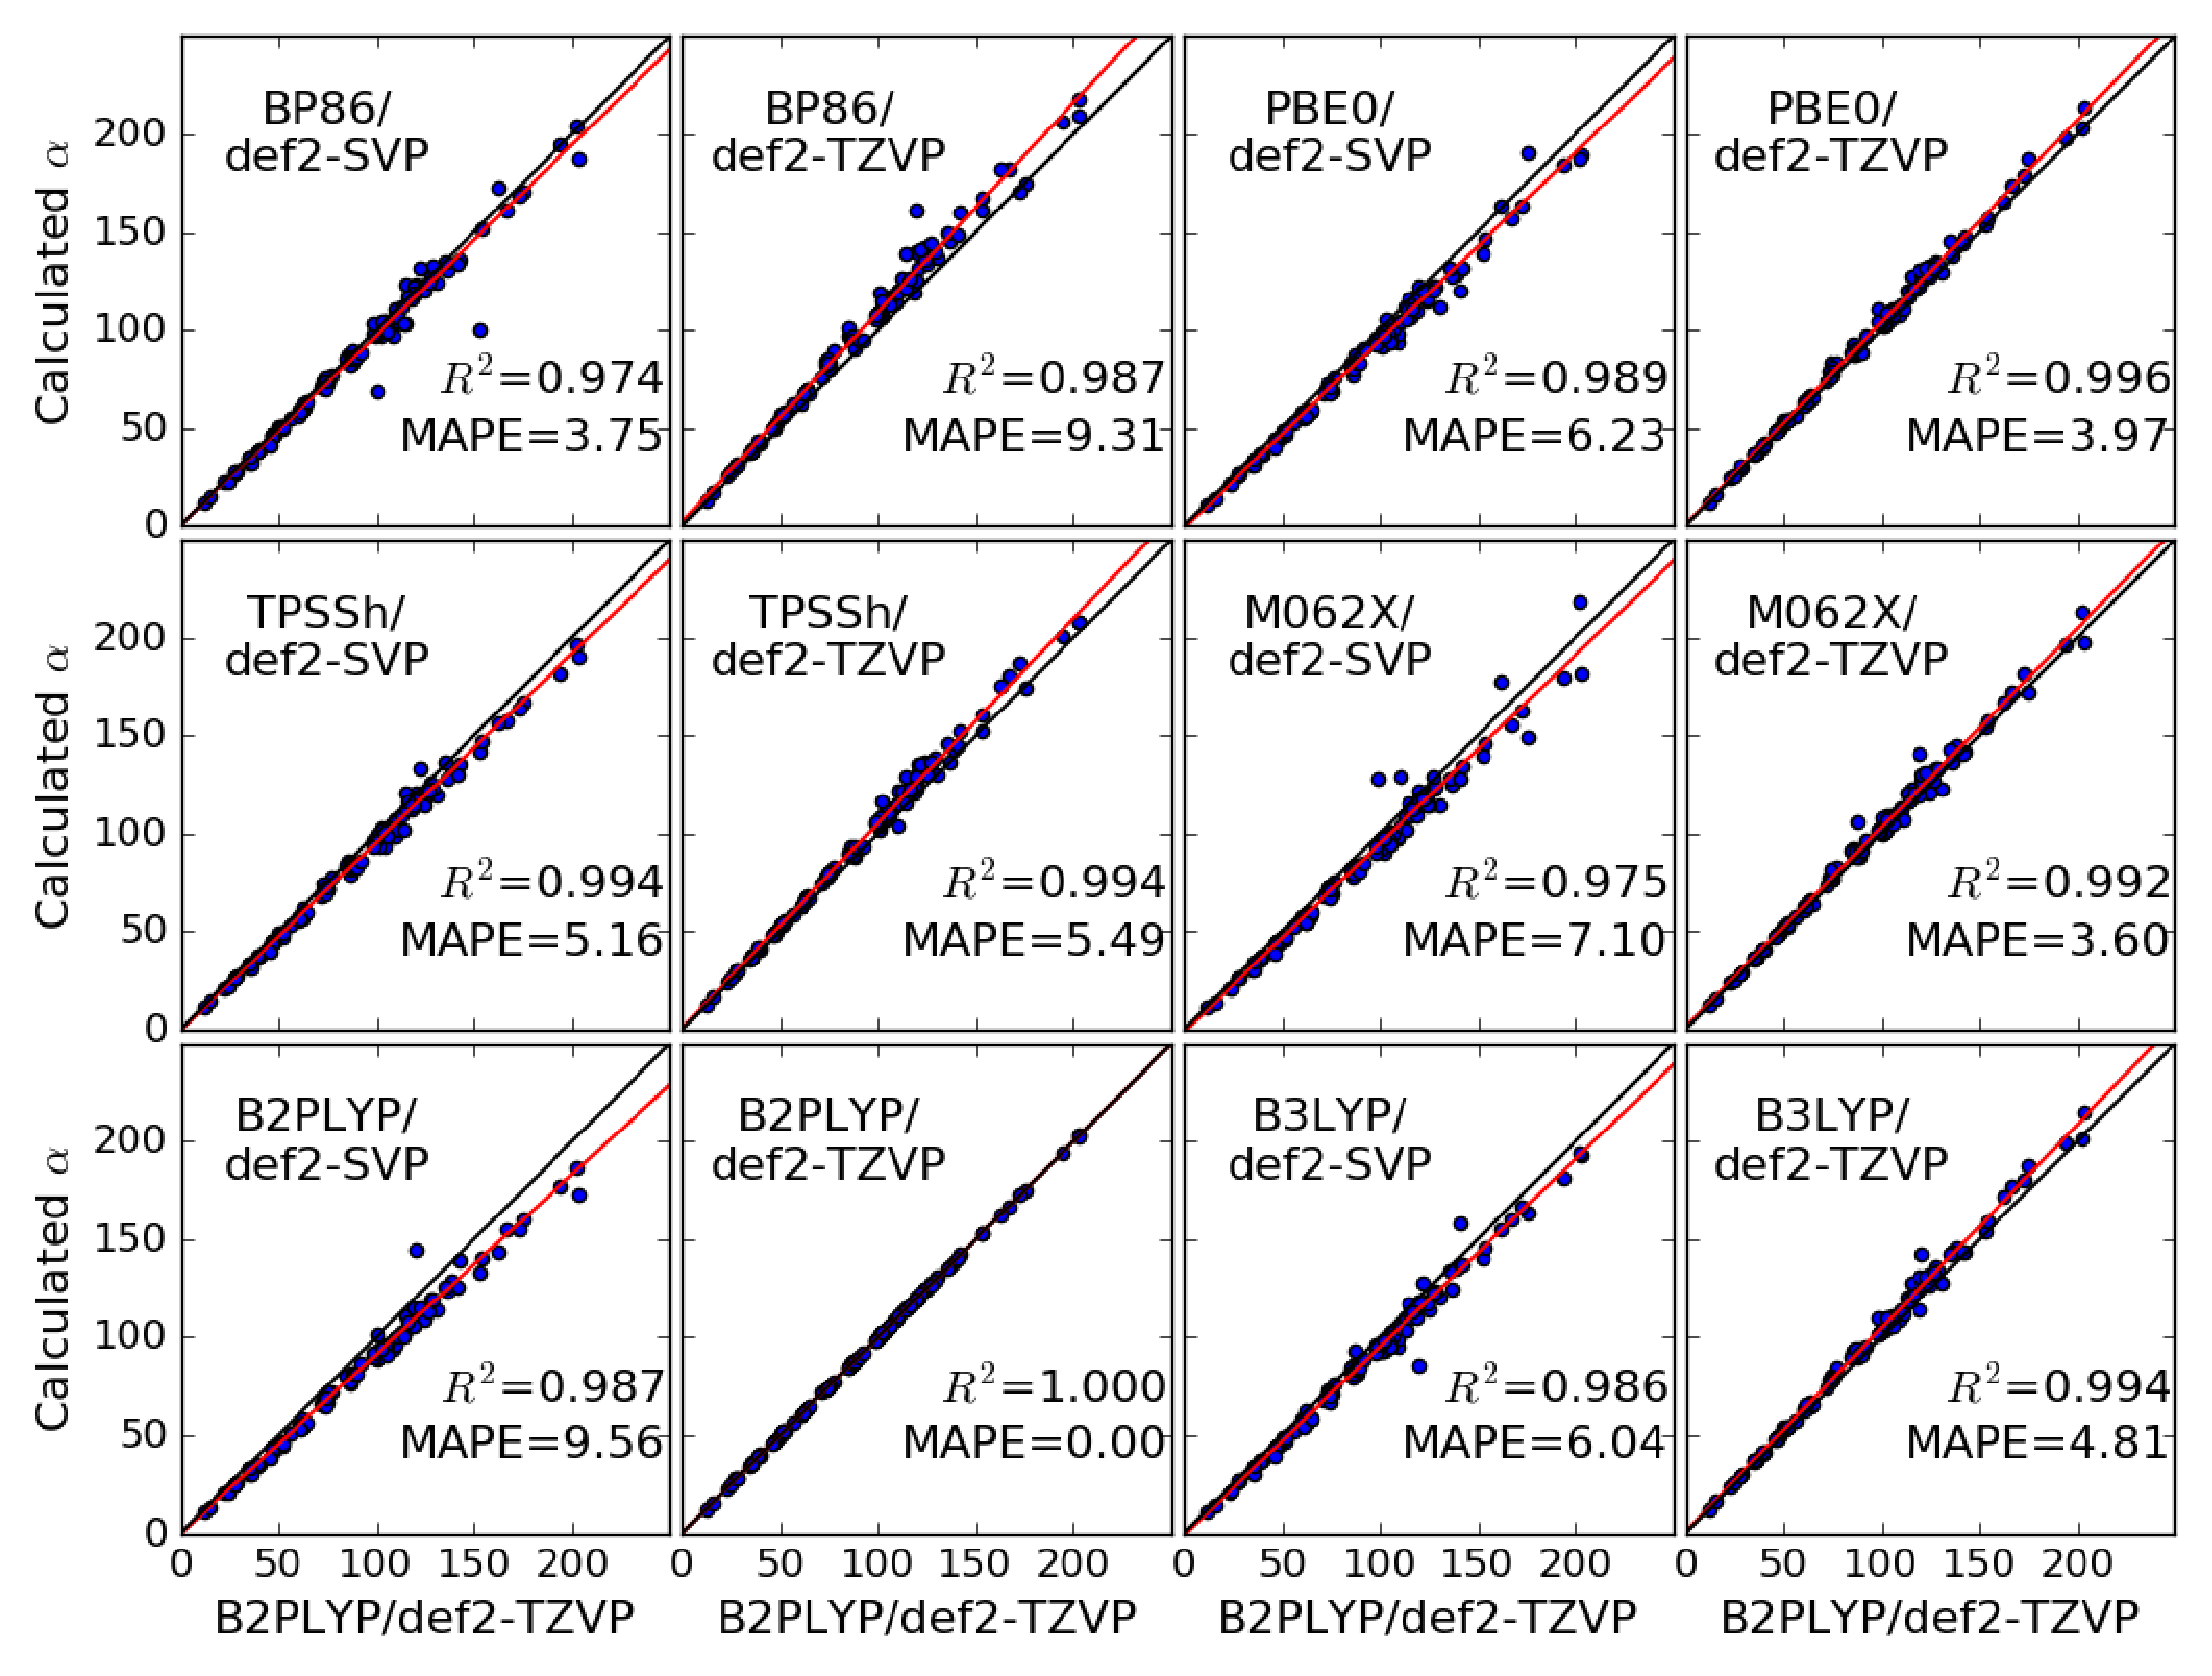
\includegraphics[width=1.00\textwidth]{Chapter-3/Figures/Pol_all_methods.eps}
	\caption{Comparison of polarizability from different methods for 112 polymers with B2PLYP/TZ as a reference.} 
	\label{fig:Pol_all_methods} 
\end{figure}  


%Comparison of polarizability from different methods for all the 112 polymers with B2PLYP/TZ as reference. Finding trends in the results. 

Fig:\ \ref{fig:Pol_all_methods} shows the performance of different model chemistries in comparison to B2PLYP/TZ. Observations from these comparisons are as follows:

\begin{itemize}
\item All the methods have a good correlation ($>$0.975) when compared with B2PLYP/TZ. However, few methods have high MAPE values ($>$5) which is caused due to an offset in the calculation as can be seen from the linear fits of the plots (red lines). For example, the linear fit of B2PLYP/DZ method below the line of symmetry (black line), as most of the values calculated from this method are lower than B2PLYP/def-TZVP. In most of the methods, the offset in the polarizability is larger for higher polarizability values. Therefore, for higher polarizability values, more accurate methods are required.
\item In all TZ calculations, the linear fit is always above the line of symmetry, whereas for all DZ calculations the linear fit is below the line of symmetry. 
\item The correlation for all TZ calculations is better when compared with the DZ calculations.
\item Among the functionals, PBE0 has the best correlation with B2PLYP/TZ and also has a lower MAPE value. Therefore, PBE0 would be a good functional to use for polarizability calculations.
\item The MAPE of B2PLYP/DZ, when compared to B2PLYP/TZ, is 9.56\%.
\end{itemize}

% Benchmarking of RI.  Mathematically discuss how the error in polarizability is translated into RI calculation
The RI ($n$) values are calculated based on the Lorentz-Lorenz equation (see eq: \ref{eqn:3}), which includes the calculation of two different properties, the polarizability ($\alpha$) and number density ($N$). To understand the error propagation from polarizability and number density to RI values, we take a logarithm on both sides of the equation and differentiate to obtain the eq: \ref{eqn:4}.  

\begin{equation} \label{eqn:3}
\frac{(n^{2}-1)}{(n^2+2)}=\frac{4\pi}{3}N\alpha
\end{equation}

\begin{equation} \label{eqn:4}
\frac{dn}{n}=\frac{(1-\frac{1}{n^2} )(1+\frac{2}{n^2})}{6}(\frac{dN}{N}+\frac{d\alpha}{\alpha})
\end{equation}

\begin{equation} \label{eqn:5}
error factor (E)=\frac{(1-\frac{1}{n^2} )(1+\frac{2}{n^2})}{6}
\end{equation}

From eq: \ref{eqn:5}, we observe that the error factor (E) is dependent only on the RI value. For the RI value ranging from 1 to 2, the value of E ranges from 0 to 0.187 respectively (see fig:\ \ref{fig:Error_factor}). Therefore, when the number density error is ignored, the error in RI calculation is less than 20\% of the error in polarizability calculation. For example, if a lower level method, BP86/def-SVP (MAPE 3.75\% compared to B2PLPY/TZ), is used to calculated polarizability instead of B2PLYP/TZ, the additional error in RI calculation would be 0.75\%. This suggests that use of lower level methods for polarizability calculations would not affect RI values significantly.

\begin{figure}[htbp]  
	\centering
	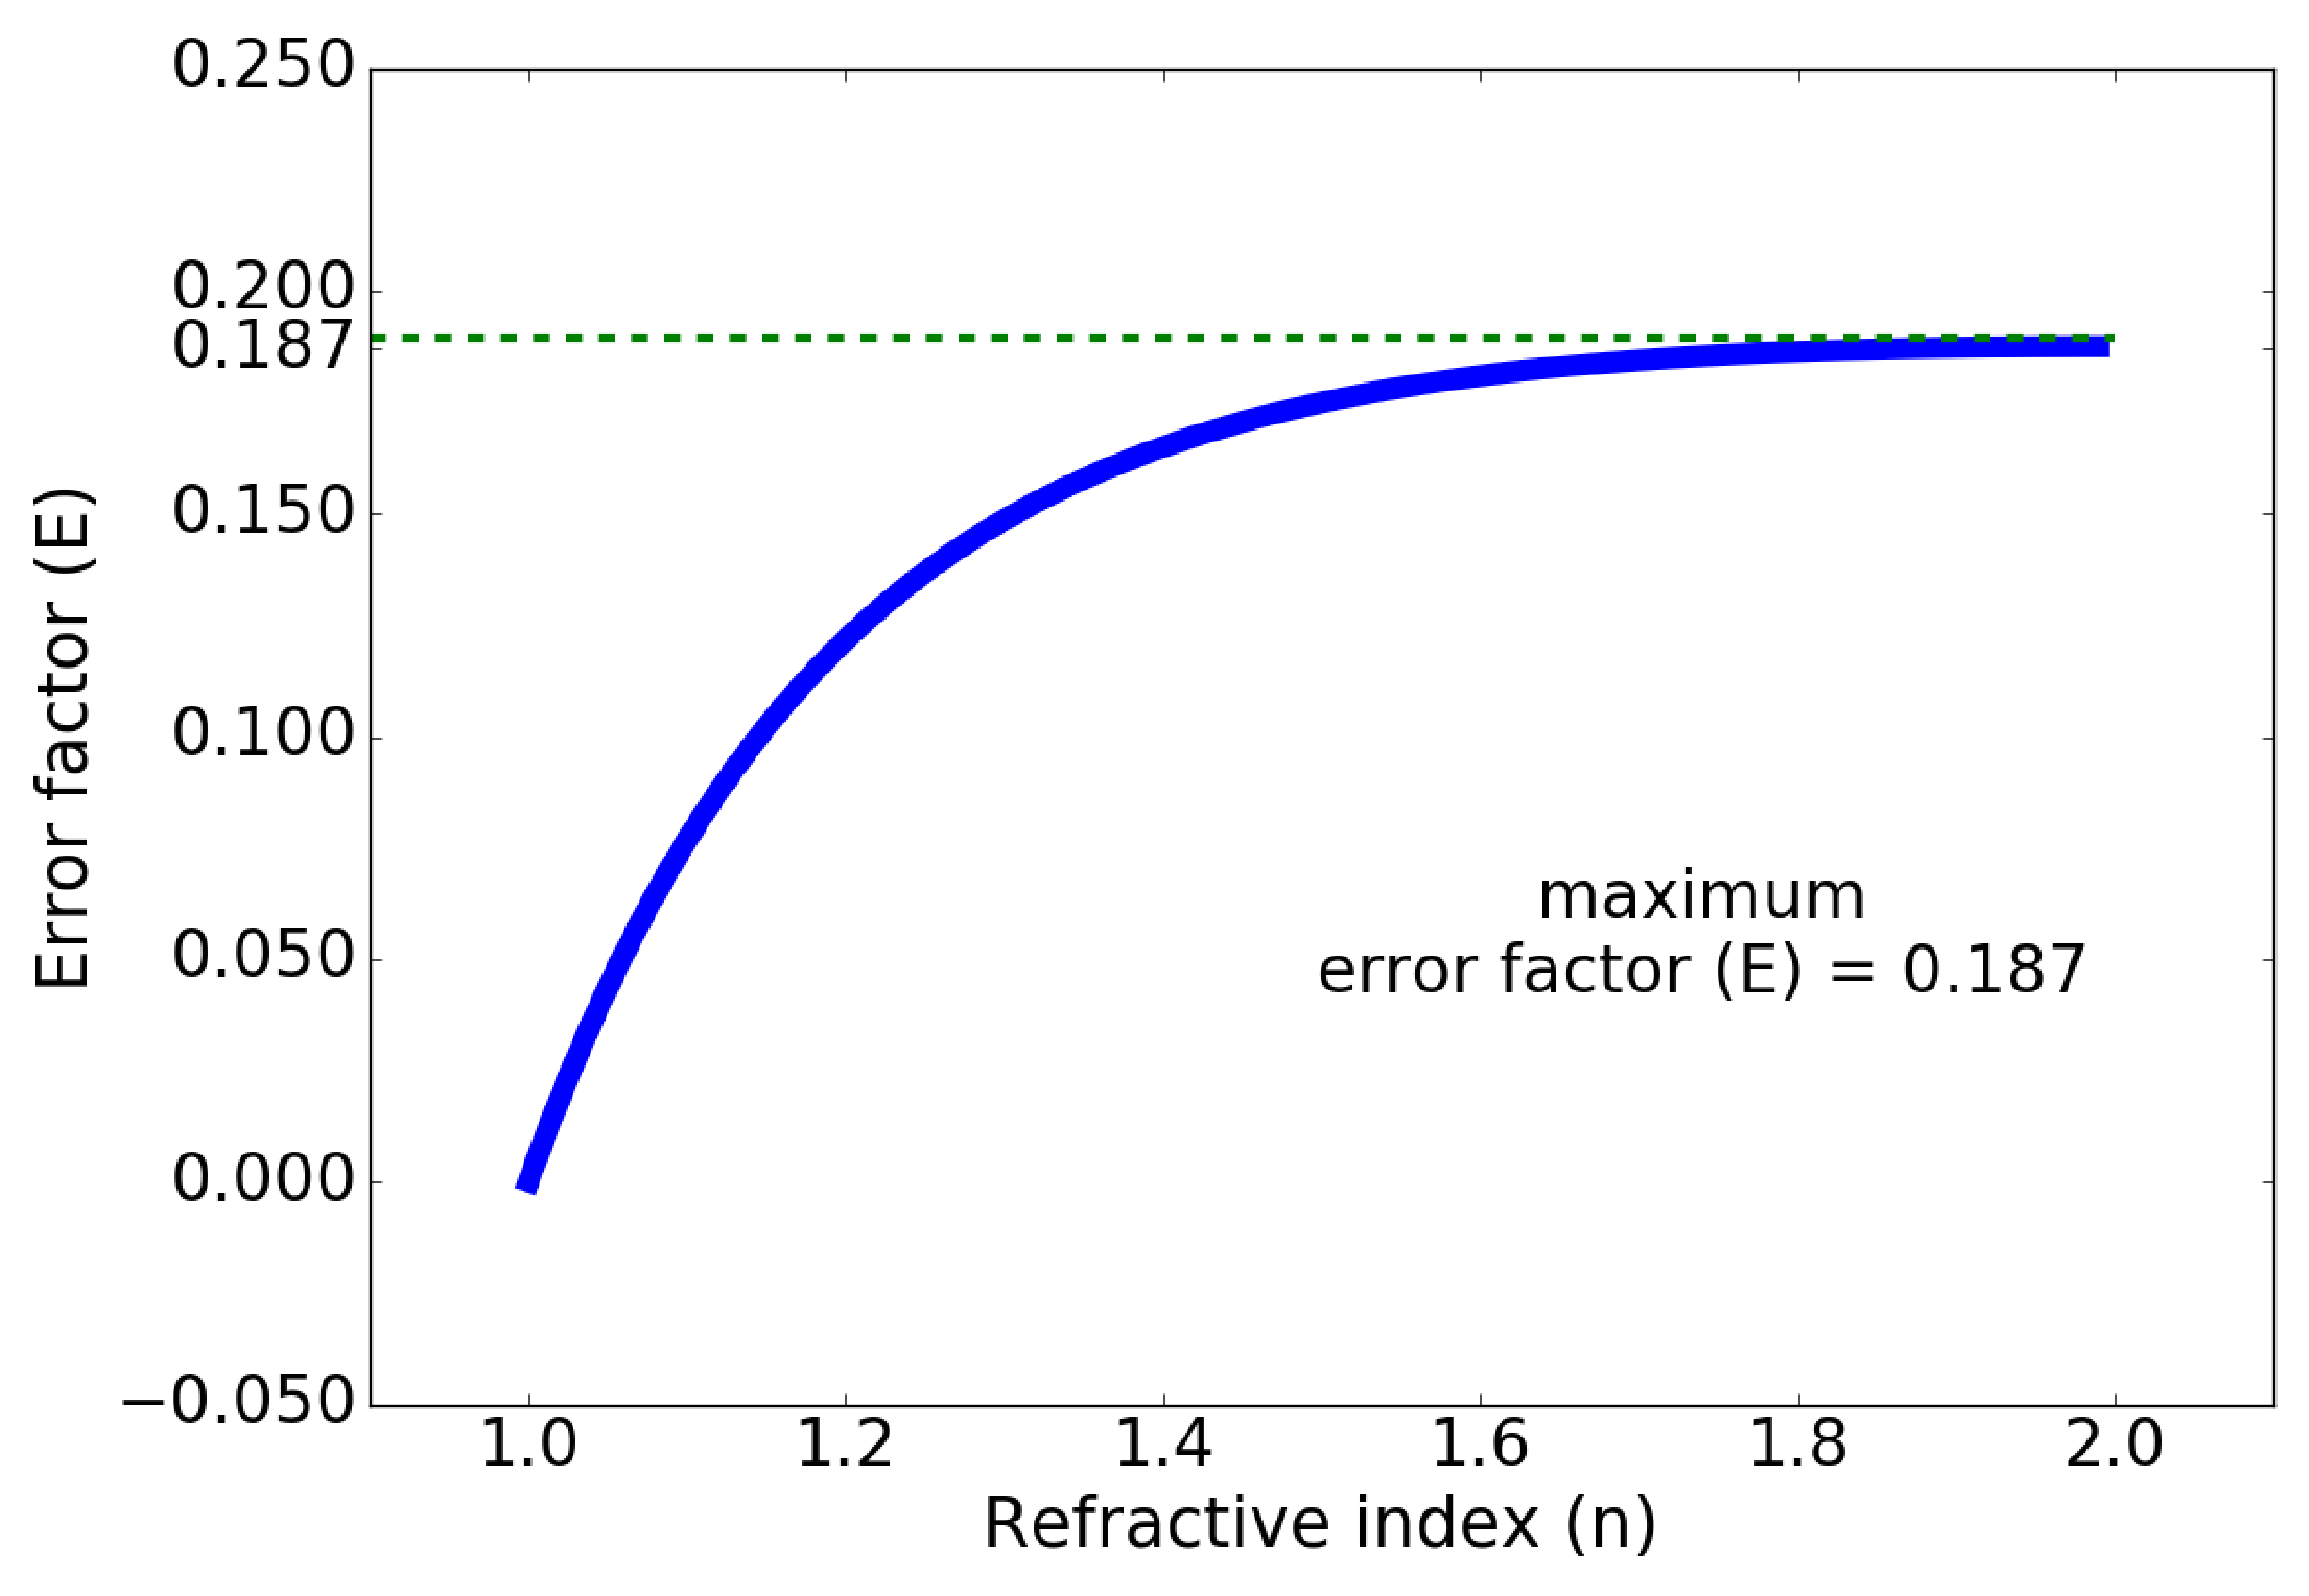
\includegraphics[width=0.744\textwidth]{Chapter-3/Figures/Error_factor.eps}
	\caption{Error factor (E) for RI values ranging from 1 to 2.} 
	\label{fig:Error_factor} 
\end{figure}  

\begin{figure}[htbp] 
	\centering
	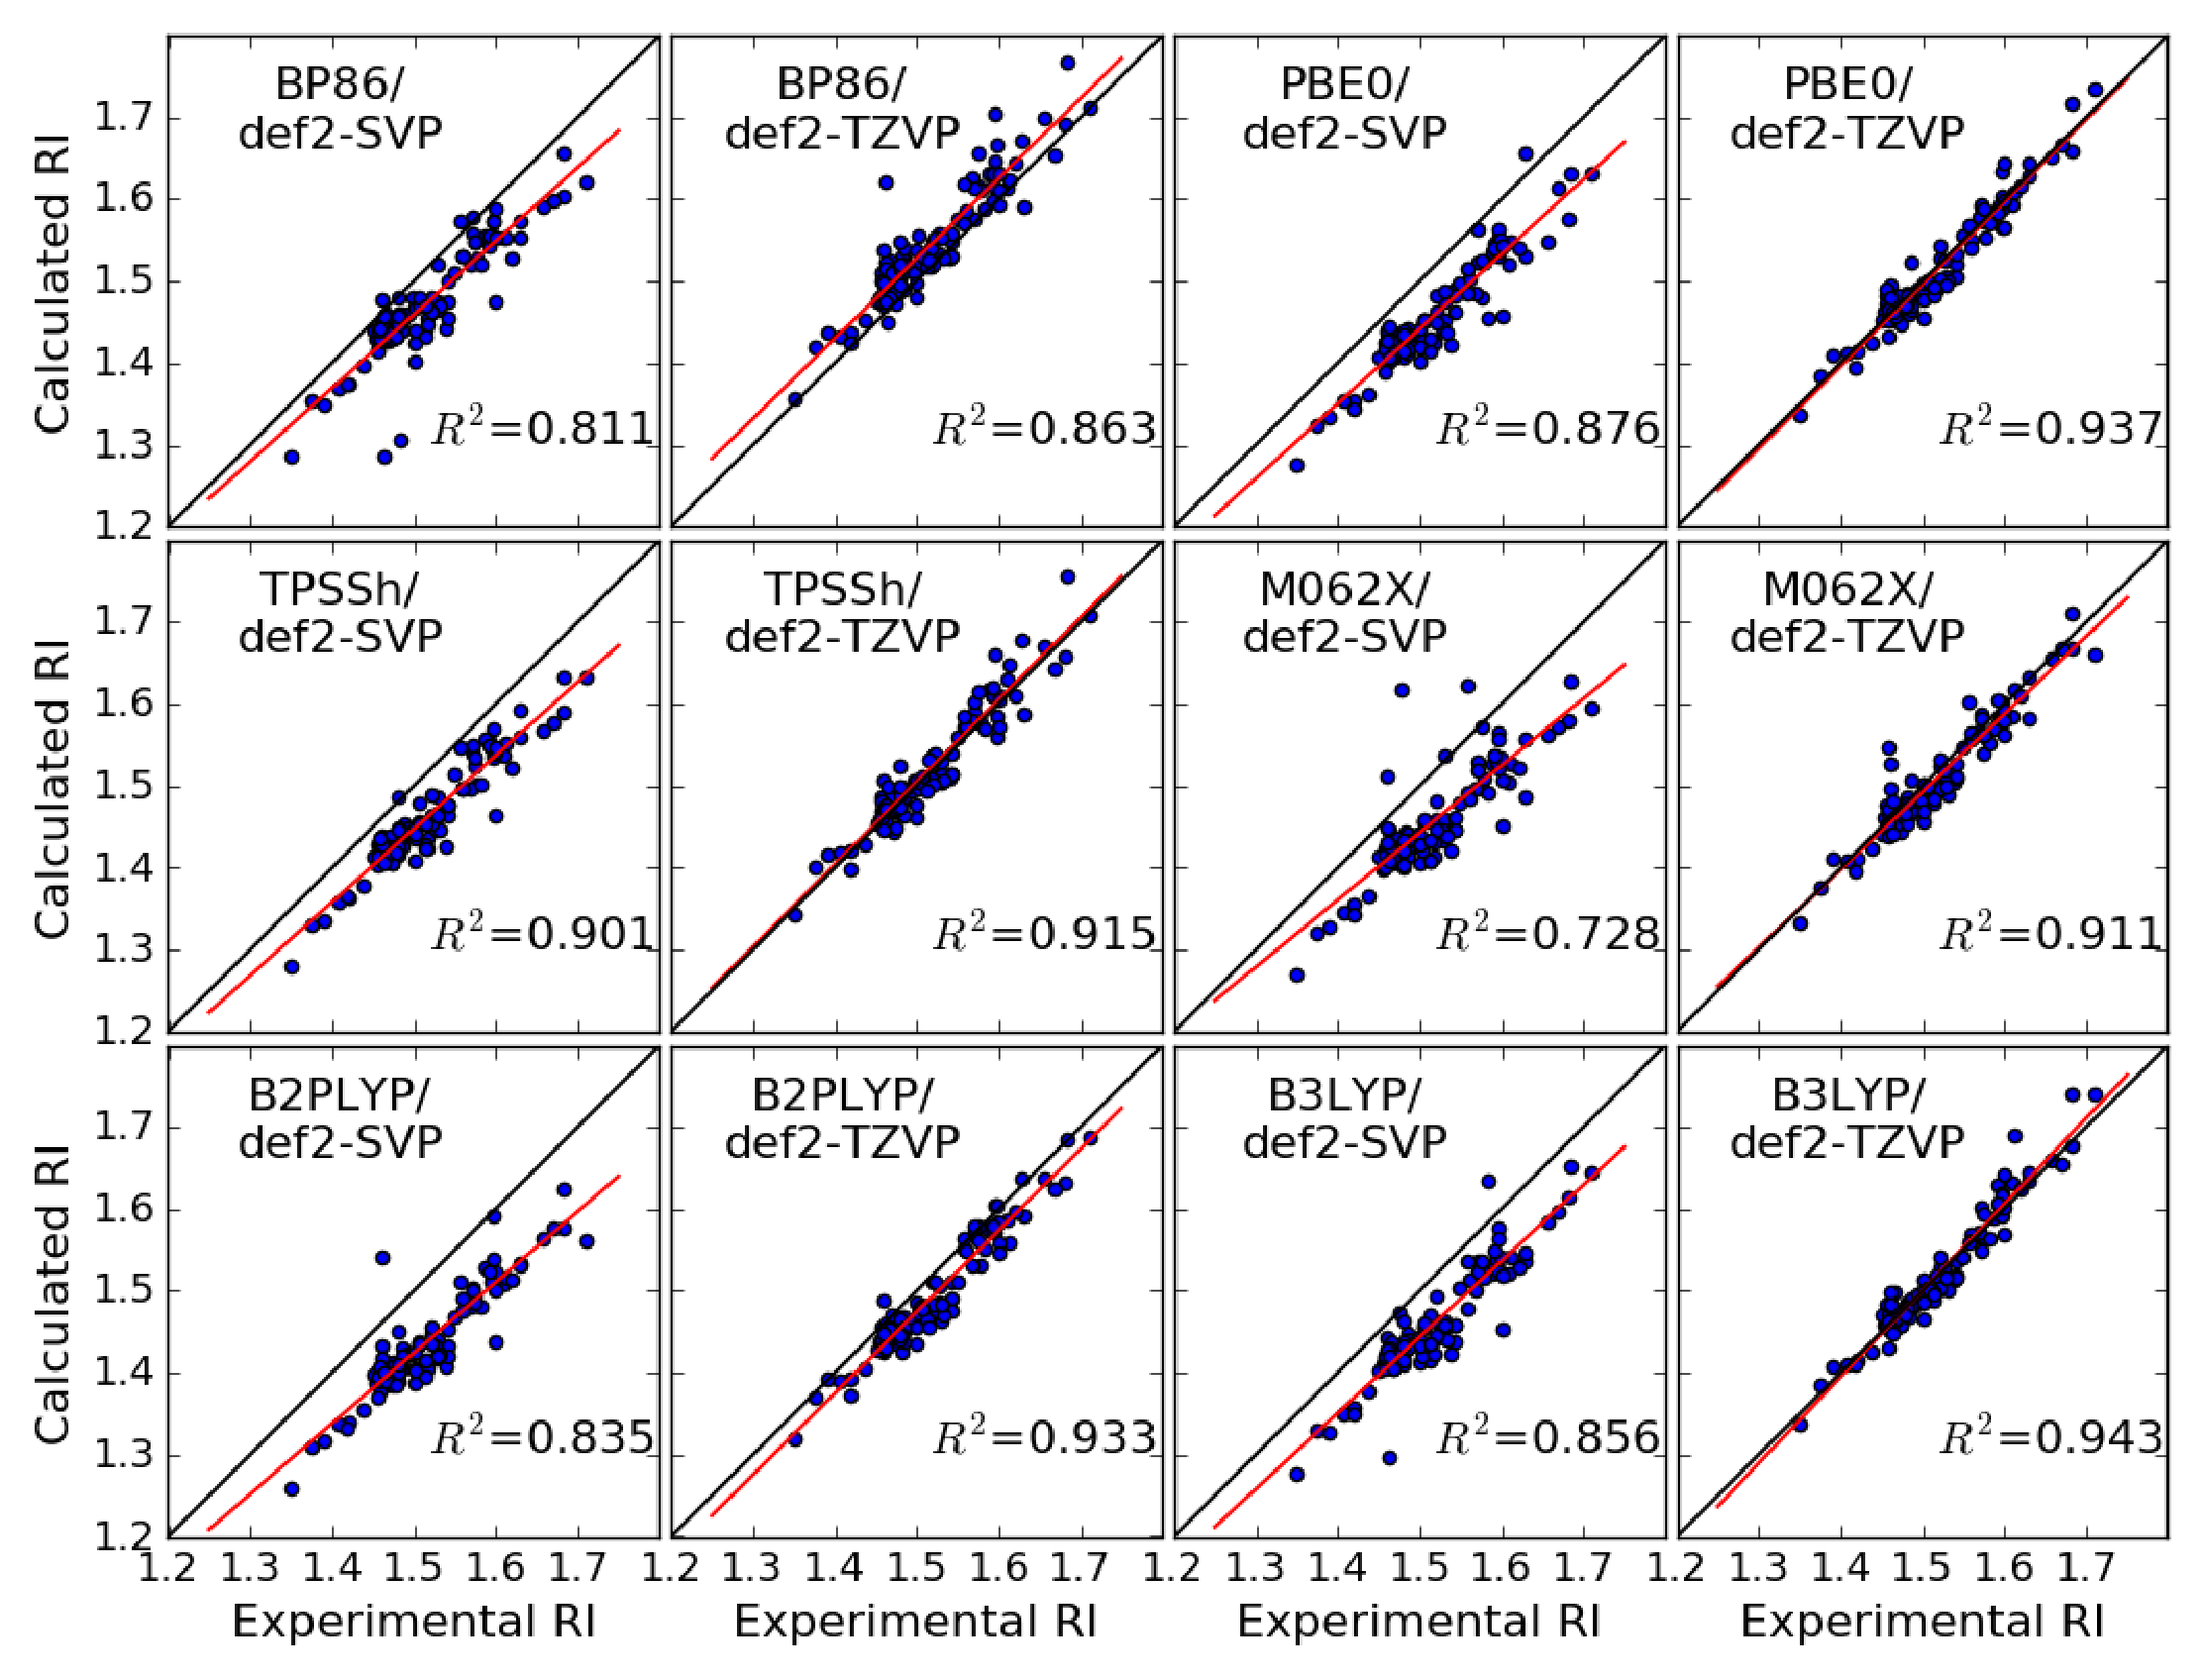
\includegraphics[width=1.00\textwidth]{Chapter-3/Figures/RI_all_methods.eps}
	\caption{Comparison of RI values calculated from different methods for 112 polymers with experimental RI values.} 
	\label{fig:RI_all_methods} 
\end{figure}  



\begin{landscape}
	\begin{table*}[t] 
		\centering
		\caption{Performance of different model chemistries in comparison to experimental values} \label{tab:1}
		\label{my-label}
		\makebox[\textwidth]{\begin{tabular}{ 	p{2.5cm}|p{1.1cm}p{1.1cm}|p{1.1cm}p{1.1cm}|p{1.1cm}p{1.1cm}|p{1.1cm}p{1.1cm}|p{1.1cm}p{1.1cm}|p{1.1cm}p{1.1cm} }
				\hline
				\textbf{Functional}    & \multicolumn{2}{c|}{\textbf{BP86}}                                                                                           & \multicolumn{2}{c|}{\textbf{PBE0}}                                                                                           & \multicolumn{2}{c|}{\textbf{TPSSh}}                                                                                          & \multicolumn{2}{c|}{\textbf{M06-2X}}                                                                                          & \multicolumn{2}{c|}{\textbf{B2PLYP}}                                                                                         & \multicolumn{2}{c}{\textbf{B3LYP}}                                                                                          \\ \hline
				\textbf{Basis set}     & \textbf{\begin{tabular}[c]{@{}c@{}}DZ\end{tabular}} & \textbf{\begin{tabular}[c]{@{}c@{}}TZ\end{tabular}} & \textbf{\begin{tabular}[c]{@{}c@{}}DZ\end{tabular}} & \textbf{\begin{tabular}[c]{@{}c@{}}TZ\end{tabular}} & \textbf{\begin{tabular}[c]{@{}c@{}}DZ\end{tabular}} & \textbf{\begin{tabular}[c]{@{}c@{}}TZ\end{tabular}} & \textbf{\begin{tabular}[c]{@{}c@{}}DZ\end{tabular}} & \textbf{\begin{tabular}[c]{@{}c@{}}TZ\end{tabular}} & \textbf{\begin{tabular}[c]{@{}c@{}}DZ\end{tabular}} & \textbf{\begin{tabular}[c]{@{}c@{}}TZ\end{tabular}} & \textbf{\begin{tabular}[c]{@{}c@{}}DZ\end{tabular}} & \textbf{\begin{tabular}[c]{@{}c@{}}TZ\end{tabular}} \\ 
				\hline
				\textbf{R$^2$} & 0.811           & 0.863           & 0.876           & 0.937           & 0.901            & 0.915           & 0.728            & 0.911           & 0.835            & 0.933            & 0.856            & 0.943           \\
				\textbf{AE}                  & 0.042           & -0.027          & 0.06            & 0.004           & 0.054            & -0.005          & 0.06             & 0.008           & 0.078            & 0.026            & 0.057            & -0.001          \\
				\textbf{MaxE}                & 0.177           & 0.159           & 0.142           & 0.045           & 0.137            & 0.073           & 0.149            & 0.088           & 0.161            & 0.068            & 0.166            & 0.077           \\
				\textbf{SPRE}                & 0.195           & 0.197           & 0.17            & 0.089           & 0.144            & 0.115           & 0.29             & 0.137           & 0.242            & 0.096            & 0.218            & 0.111           \\
				\textbf{MAE}                 & 0.043           & 0.029           & 0.06            & 0.014           & 0.054            & 0.016           & 0.065            & 0.017           & 0.079            & 0.027            & 0.058            & 0.013           \\
				\textbf{MARE}                & 0.028           & 0.019           & 0.04            & 0.009           & 0.036            & 0.011           & 0.042            & 0.011           & 0.052            & 0.018            & 0.038            & 0.008           \\
				\textbf{RMSD}                & 0.052           & 0.038           & 0.064           & 0.018           & 0.058            & 0.021           & 0.07             & 0.022           & 0.082            & 0.031            & 0.063            & 0.018           \\
				\textbf{RMSRE}               & 0.042           & 0.031           & 0.052           & 0.014           & 0.047            & 0.017           & 0.056            & 0.018           & 0.067            & 0.025            & 0.051            & 0.014           \\
				\textbf{Slope}               & 0.9             & 0.98            & 0.91            & 1               & 0.9              & 1               & 0.82             & 0.95            & 0.86             & 0.99             & 0.93             & 10.05            \\
				\textbf{Intercept}           & 0.11            & 0.06            & 0.07            & -0.01           & 0.1              & 0               & 0.21             & 0.07            & 0.13             & -0.02            & 0.05             & -0.08          
			\end{tabular}}
		\end{table*}
	\end{landscape}

%Calculating RI and comparing with experimental results of RI of these polymers.
The RI values for the 112 polymers is calculated using six functionals (BP86, PBE0, TPSSh, M06-2X, B2PLY and B3LYP) and two basis sets (DZ and TZ). The correlation with experimental values and the error analysis of each of these methods is shown in the table \ref{tab:1}. 

Observations:

i. In all the cases, TZ calculations are better than the DZ calculations. 

ii. The functionals B2PLYP, B3LYP and PBE0 have relatively better performance, whereas the M06-2X functional has the worst performance. 

iii. Comparing all the methods, the $R^2$ value for B3LYP/TZ is the highest. This method also has the lowest AE, MAE and MARE. However, the lowest maximum error is observed for PBE0/TZ. 

iv. All the methods showed a maximum error less than 0.2, with a lowest error of 0.045 for PBE0/TZ. Further, the SPR error for this method is 0.089, which suggests that this method is accurate for RI calculation. 

v. If only DZ is considered, then PBE0 and TPSSh functionals have the better performance compared to other functionals. 

vi. The slope and intercept of the linear correlations for the methods TPSSh/TZ, B2PLYP/TZ and PBE0/TZ are 1 and 0 respectively, suggesting that the linear correlation is exact. This can be observed in Fig.\ \ref{fig:RI_all_methods}, where the linear fit (red line) overlaps the line of symmetry (black line).  Thus, the calculated values do not have to be corrected by a factor for these methods. For all the other methods except B3LYP/TZ, the slope is less than 1, which shows that these methods under-predict the RI of polymers with high RI values.

vii. Considering the time of calculations v/s the accuracy of the methods, PBE0/DZ and TPSSh/DZ show the best promise for RI calculation. 

%Discussion on how these benchmarking results will enhance the performance in terms of high-throughput screening of potential candidates.
Now that we have developed a robust protocol for RI prediction of polymers, our next step is to cast these into our automated high-throughput framework, and employ in on an extensive candidate screening library. We plan to apply this framework to discover high RI polyimides and polyenes. The candidate library of these polymers will be created from promising building blocks using our combinatorial library generator. We will also pursue the development of a smart, responsive, and thus more efficient scheme in the course of the project, which will avoid the problems of exponential growth. The different screening phases will successively reduce the pool of viable candidates. The resulting data will be analyzed, mined, and modeled using machine learning and informatics techniques to extract structure-property relationships.



% ...

\section{Conclusions}
\label{sec:conclusions3}

We have successfully created 270,000 novel PI candidates, and evaluated the RI values of these candidates by casting into \chemhtps. From the screening studies, we found PI candidates that possess RI values greater than 1.8. 
Z-score analysis showed that prevalence of certain building blocks ( \eg building blocks 25 and 28) in a top candidates. In addition to identifying individual building blocks that are promising for high RI polymers, promising building block pairs are also identified.  Z-score value. We observed that the combination of building block 28 with blocks 2 and 3 to be highly promising in the design of HRIPs. Thus, we successfully identified favorable building blocks and synergy between building blocks combinations for developing high RI PIs. We demonstrated that our cyberinfrastructure is a powerful tool and has shown to be highly promising for identifying polyimides with exceptional RI values.